\documentclass[ngerman,a4paper,order=firstname]{../../texmf/tex/latex/mathscript/mathscript}
\usepackage{../../texmf/tex/latex/mathoperators/mathoperators}

\title{\textbf{Programmieren für Mathematiker SS2018}}
\author{Dozent: Prof. Dr. Wolfgang Walter}

\begin{document}
\pagenumbering{roman}
\pagestyle{plain}

\maketitle

\hypertarget{tocpage}{}
\tableofcontents
\bookmark[dest=tocpage,level=1]{Inhaltsverzeichnis}

\pagebreak
\pagenumbering{arabic}
\pagestyle{fancy}

\chapter*{Vorwort}
Schön, dass du unser Skript für die Vorlesung \textit{Lineare Algebra und analytische Geometrie 1} bei Prof. Dr. Arno Fehm im WS2017/18 gefunden hast! \footnote{Obwohl man sagen kann, dass es in dieser Vorlesung nur um Lineare Algebra ging, der Teil mit der analytischen Geometrie wurde vernachlässigt. Liegt wahrscheinlich auch daran, dass es demnächst eine Reform der Studienordnung gibt, in der aus der Vorlesung \textit{Lineare Algebra und analytische Geometrie} die Vorlesung \textit{Einführung in die Lineare Algebra} wird.}

Wir verwalten dieses Skript mittels Github \footnote{Github ist eine Seite, mit der man Quelltext online verwalten kann. Dies ist dahingehend ganz nützlich, dass man die Quelltext-Dateien relativ einfach miteinander synchronisieren kann, wenn man mit mehren Leuten an einem Projekt arbeitet.}, d.h. du findest den gesamten \LaTeX-Quelltext auf \url{https://github.com/henrydatei/TUD_MATH_BA}. Unser Ziel ist, für alle Pflichtveranstaltungen von \textit{Mathematik-Bachelor} ein gut lesbares Skript anzubieten. Für die Programme, die in den Übungen zur Vorlesung \textit{Programmieren für Mathematiker} geschrieben werden sollen, habe ich ein eigenes Repository eingerichtet; es findet sich bei \url{https://github.com/henrydatei/TU_PROG}.

Du kannst dir gerne dort die \LaTeX-Quelldateien herunterladen, die Dateien für exakt dieses Skript sind im Ordner \texttt{1. Semester/LAAG ueberarbeitet}. Es lohnt sich auf jeden Fall während des Studiums die Skriptsprache \LaTeX{} zu lernen, denn Dokumente, die viele mathematische oder physikalische Formeln enthalten, lassen sich sehr gut mittels \LaTeX{} darstellen, in Word oder anderen Office-Programmen sieht so etwas dann eher dürftig aus.

\LaTeX{} zu lernen ist gar nicht so schwierig, ich habe dafür am Anfang des ersten Semesters wenige Wochen benötigt, dann kannte ich die wichtigsten Befehle und konnte den Vorgänger dieses Skriptes schreiben (\texttt{1. Semester/LAAG}, Vorsicht: hässlich, aber der Quelltext ist relativ gut verständlich).

Es sei an dieser Stelle darauf hingewiesen (wie in jedem anderem Skript auch \smiley{}), dass dieses Skript nicht den Besuch der Vorlesungen ersetzen kann. Es könnte sein, dass Prof. Fehm seine Vorlesung immer mal wieder an die Studenten anpasst; wahrscheinlich immer dann, wenn die Prüfungsergebnisse zu schlecht waren. Nichtsdestotrotz veröffentlicht Prof. Fehm sein Skript auf seiner Homepage \url{http://www.math.tu-dresden.de/~afehm/lehre.html}. Allerdings ist dieses Skript recht hässlich, besonders was die Übersichtlichkeit angeht.

Wir möchten deswegen ein Skript bereitstellen, dass zum einen übersichtlich ist, zum anderen \textit{alle} Inhalt aus der Vorlesung enthält, das sind insbesondere Diagramme, die sich nicht im offiziellen Skript befinden, aber das Verständnis des Inhalts deutlich erleichtern. Ich denke, dass uns dies erfolgreich gelungen ist.

Trotz intensivem Korrekturlesen können sich immer noch Fehler in diesem Skript befinden. Es wäre deswegen ganz toll von dir, wenn du auf unserer Github-Seite \url{https://github.com/henrydatei/TUD_MATH_BA} ein neues Issue erstellst und damit auch anderen hilfst, dass dieses Skript immer besser wird.

\chapter{Pointer}
\section{Allgemeines über Pointer}

Pointer nennt man auch \begriff{Zeiger}, \begriff{Verweise} oder \begriff{Datenreferenzen}. Ein Pointer ist ein Verweis bzw. eine Referenz auf ein Zielobjekt/Zeigerziel/Target eines festgelegten Datentyps. In den folgenden Darstellungen ist:
\begin{center}
	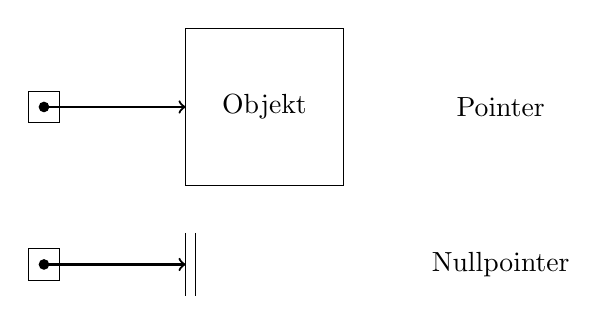
\begin{tikzpicture}[scale=0.2]
		\draw (0,0) -- (2,0);
		\draw (0,0) -- (0,2);
		\draw (2,0) -- (2,2);
		\draw (0,2) -- (2,2);
		\draw[fill = black] (1,1) circle (0.3);
		\draw[->, thick] (1,1) -- (10,1);
		\draw (10,-4) -- (10,6);
		\draw (10,-4) -- (20,-4);
		\draw (10,6) -- (20,6);
		\draw (20,-4) -- (20,6);
		\node at (15,1) (n) {Objekt};
		\node at (30,1) (n2) {Pointer};
		
		\draw (0,-10) -- (2,-10);
		\draw (0,-10) -- (0,-8);
		\draw (2,-10) -- (2,-8);
		\draw (0,-8) -- (2,-8);
		\draw[fill = black] (1,-9) circle (0.3);
		\draw[->, thick] (1,-9) -- (10,-9);
		\draw (10,-7) -- (10,-11);
		\draw (10.6,-7) -- (10.6,-11);
		\node at (30,-9) (n2) {Nullpointer};
	\end{tikzpicture}
\end{center}

Ein Pointer hat zu Beginn der Programmausführung einen undefinierten Zustand, der nicht als solcher erkannt werden kann. Die Verwendung eines solchen Pointers kann große Probleme verursachen.

Zeiger sind kein eigenständiger Typ, sondern nur mit dem Attribut \texttt{pointer} gekennzeichnet:
\begin{lstlisting}
! eine normale Variable
integer :: variable
! ein Pointer
integer, pointer :: ptr
\end{lstlisting}

Zeiger sind streng typisiert, das heißt man kann nur auf Objekte zeigen, deren Typ identisch mit dem Zeigertyp ist. Es gibt also keine Universalpointer. Der Pointer im oberen Quelltext kann also nur auf Variablen mit dem Typ \texttt{integer} zeigen.

Jedes beliebige Objekt vom passenden Objekttyp kann als Ziel eines Zeigers dieses Typs verwendet werden, wenn die Zielvariable das Attribut \texttt{target} trägt oder das Objekt ein dynamisches im Heap erzeugtes Objekt ist.
\begin{lstlisting}
integer, target :: ziel
integer, pointer :: ptr
\end{lstlisting}

Jede Pointer-Variable kann als Zeigerziel dienen. Ohne \texttt{target}-Attribut.

Implizit werden Pointer immer automatisch dereferenziert, außer in den Anweisungen \texttt{nullify()}, \texttt{allocate()}, \texttt{deallocate()}, der Pointer-Zuweisung \texttt{pointer => ziel} sowie in der \texttt{associated}-Abfragefunktion.

Pointer sind in Fortran in der Regel mehr als nur Adressen.

Werfen wir nun nochmal einen Blick auf die Pointer-Kontexte, in denen Pointer automatisch dereferenziert werden.

\begin{*anmerkung}
	Wird gerne in der Klausur abgefragt, steht aber auch in dem zur Klausur zugelassenen Buch des Rechenzentrums Niedersachsen über den Fortran-Standard.
\end{*anmerkung}

\begin{itemize}
	\item Die Funktion \texttt{nullify(p1, p2, ...)} versetzt die Pointer \texttt{p1}, \texttt{p2} und so weiter in den definierten Zustand Null = nicht assoziiert.
	\item \texttt{allocate(p1, p2, ...)} legt Speicherblöcke im Heap für die Zielobjekte der Pointer an und setzt die Pointer als Referenzen auf ihren jeweiligen Speicherblock. Alle Pointer sind im definierten Zustand assoziiert.
	\item Mit \texttt{deallocate(p1, p2, ...)} werden die Speicherblöcke, auf die die Pointer zeigen freigegeben und die Pointer auf Null gesetzt. Der Pointer muss dafür assoziiert und ein ganzen Objekt, also kein Subarray, Substring oder ähnliches, sein.
	\item Pointer werden mit \texttt{ptr => tgt} oder \texttt{ptr1 => ptr2} zugewiesen.
	\item Die Abfragefunktion \texttt{associated()} kann auf recht unterschiedliche Weisen eingesetzt werden:
	\begin{itemize}
		\item \texttt{associated(ptr)} $\to$ \texttt{.true.}, wenn auf ein Ziel gezeigt wird; \texttt{.false.}, wenn \texttt{ptr} auf Null zeigt.
		\item \texttt{associated(ptr, tgt)} $\to$ \texttt{.true.}, wenn \texttt{ptr} auf \texttt{tgt} zeigt, sonst \texttt{.false.}
		\item \texttt{associated(ptr1, ptr2)} $\to$ \texttt{.true.}, wenn beide Pointer denselben Zustand (nicht Null) haben, sonst \texttt{.false.}
	\end{itemize}
\end{itemize}

Wie schon oben angesprochen, ist der Umgang mit Pointern nicht ganz ungefährlich, es gibt einige Gefahren für den Hauptspeicher, insbesondere den Heap.

\begin{*anmerkung}
	auch wichtig in der Klausur, steht aber leider nicht im Buch, muss also auswendig gelernt werden
\end{*anmerkung}

\begin{itemize}
	\item Verwendung eines nicht definierten oder nicht gültigen Pointers in \texttt{deallocate}, \texttt{=>}, \texttt{associated}-Abfragen und normalen (nicht Pointer-) Kontext, das heißt in Expressions, in denen alle Pointer automatisch dereferenziert werden.
	\item \begriff{Dangling Pointer} entstehen, wenn das Zeigerziel verloren geht, z.B. durch \texttt{deallocate} über anderen Pointern oder eines \texttt{allocatable}-Feldes oder wenn das Zielobjekt "'out of scope"' geht, zum Beispiel durch Verlassen seiner Prozedur.
	\item \begriff{Speicherleichen}, Garbage, memory leaks: haben im Prinzip das ewige Leben im Heap, wenn keine Referenzen mehr auf ein Heap-Objekt existiert, über die man es freigeben könnte.
\end{itemize}
\section{Listen}

Eine \begriff{Liste} ist eine lineare Anordnung von Objekten des selben Typs. Eine Liste wird als verzeigerte Struktur (oder als eindimensionales Feld - wird hier aber nicht behandelt) implementiert. Eine solche Liste hat 3 Attribute:
\begin{itemize}
	\item linear vs. zyklisch
	\item einfach verkettet vs. doppelt verkettet
	\item endogen vs. exogen
\end{itemize}

\begin{center}
	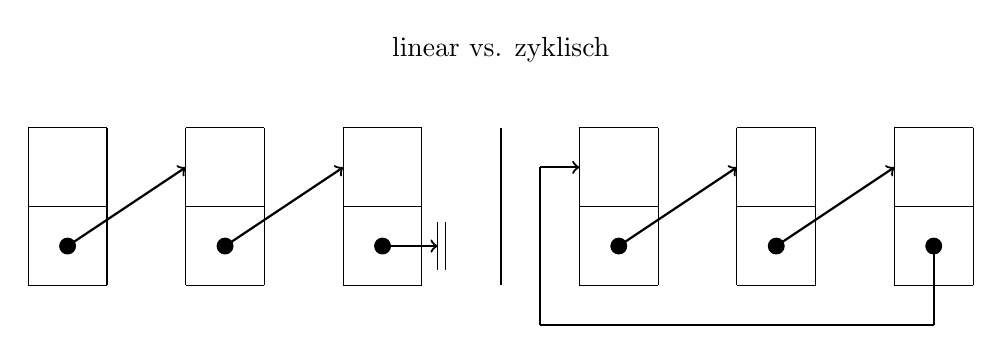
\begin{tikzpicture}
		\node at (0,0) (lz) {linear vs. zyklisch};
		\draw (-4,-1) -- (-3,-1);
		\draw (-4,-3) -- (-3,-3);
		\draw (-4,-1) -- (-4,-3);
		\draw (-3,-1) -- (-3,-3);
		\draw (-4,-2) -- (-3,-2);
		\draw[fill=black] (-3.5,-2.5) circle (0.1);
		\draw[->, thick] (-3.5,-2.5) -- (-2,-1.5);
		\draw (-6,-1) -- (-5,-1);
		\draw (-6,-3) -- (-5,-3);
		\draw (-6,-1) -- (-6,-3);
		\draw (-5,-1) -- (-5,-3);
		\draw (-6,-2) -- (-5,-2);
		\draw[fill=black] (-5.5,-2.5) circle (0.1);
		\draw[->, thick] (-5.5,-2.5) -- (-4,-1.5);
		\draw (-2,-1) -- (-1,-1);
		\draw (-2,-3) -- (-1,-3);
		\draw (-2,-1) -- (-2,-3);
		\draw (-1,-1) -- (-1,-3);
		\draw (-2,-2) -- (-1,-2);
		\draw[fill=black] (-1.5,-2.5) circle (0.1);
		\draw[->, thick] (-1.5,-2.5) -- (-0.8,-2.5);
		\draw (-0.8,-2.2) -- (-0.8,-2.8);
		\draw (-0.7,-2.2) -- (-0.7,-2.8);
		
		\draw[thick] (0,-1) -- (0,-3);
		
		\draw (4,-1) -- (3,-1);
		\draw (4,-3) -- (3,-3);
		\draw (4,-1) -- (4,-3);
		\draw (3,-1) -- (3,-3);
		\draw (4,-2) -- (3,-2);
		\draw[fill=black] (3.5,-2.5) circle (0.1);
		\draw[->, thick] (1.5,-2.5) -- (3,-1.5);
		\draw (6,-1) -- (5,-1);
		\draw (6,-3) -- (5,-3);
		\draw (6,-1) -- (6,-3);
		\draw (5,-1) -- (5,-3);
		\draw (6,-2) -- (5,-2);
		\draw[fill=black] (5.5,-2.5) circle (0.1);
		\draw[->, thick] (3.5,-2.5) -- (5,-1.5);
		\draw (2,-1) -- (1,-1);
		\draw (2,-3) -- (1,-3);
		\draw (2,-1) -- (2,-3);
		\draw (1,-1) -- (1,-3);
		\draw (2,-2) -- (1,-2);
		\draw[fill=black] (1.5,-2.5) circle (0.1);
		\draw[thick] (5.5,-2.5) -- (5.5,-3.5);
		\draw[thick] (5.5,-3.5) -- (0.5,-3.5);
		\draw[thick] (0.5,-3.5) -- (0.5,-1.5);
		\draw[->, thick] (0.5,-1.5) -- (1,-1.5);
	\end{tikzpicture}
\end{center}

\begin{center}
	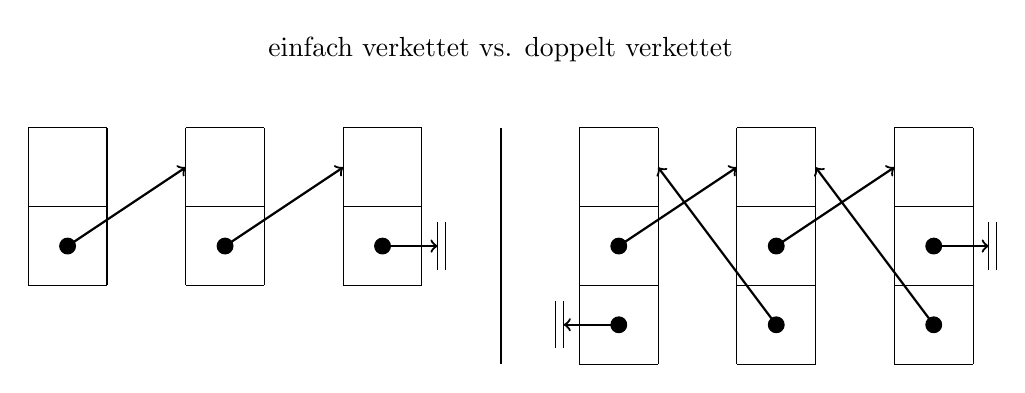
\begin{tikzpicture}
		\node at (0,0) (lz) {einfach verkettet vs. doppelt verkettet};
		\draw (-4,-1) -- (-3,-1);
		\draw (-4,-3) -- (-3,-3);
		\draw (-4,-1) -- (-4,-3);
		\draw (-3,-1) -- (-3,-3);
		\draw (-4,-2) -- (-3,-2);
		\draw[fill=black] (-3.5,-2.5) circle (0.1);
		\draw[->, thick] (-3.5,-2.5) -- (-2,-1.5);
		\draw (-6,-1) -- (-5,-1);
		\draw (-6,-3) -- (-5,-3);
		\draw (-6,-1) -- (-6,-3);
		\draw (-5,-1) -- (-5,-3);
		\draw (-6,-2) -- (-5,-2);
		\draw[fill=black] (-5.5,-2.5) circle (0.1);
		\draw[->, thick] (-5.5,-2.5) -- (-4,-1.5);
		\draw (-2,-1) -- (-1,-1);
		\draw (-2,-3) -- (-1,-3);
		\draw (-2,-1) -- (-2,-3);
		\draw (-1,-1) -- (-1,-3);
		\draw (-2,-2) -- (-1,-2);
		\draw[fill=black] (-1.5,-2.5) circle (0.1);
		\draw[->, thick] (-1.5,-2.5) -- (-0.8,-2.5);
		\draw (-0.8,-2.2) -- (-0.8,-2.8);
		\draw (-0.7,-2.2) -- (-0.7,-2.8);
		
		\draw[thick] (0,-1) -- (0,-4);
		
		\draw (4,-1) -- (3,-1);
		\draw (4,-3) -- (3,-3);
		\draw (4,-1) -- (4,-3);
		\draw (3,-1) -- (3,-3);
		\draw (4,-2) -- (3,-2);
		\draw[fill=black] (3.5,-2.5) circle (0.1);
		\draw[->, thick] (1.5,-2.5) -- (3,-1.5);
		\draw (4,-3) -- (4,-4);
		\draw (4,-4) -- (3,-4);
		\draw (3,-4) -- (3,-3);
		\draw[fill=black] (3.5,-3.5) circle (0.1);
		\draw[->, thick] (3.5,-3.5) -- (2,-1.5);
		\draw (6,-1) -- (5,-1);
		\draw (6,-3) -- (5,-3);
		\draw (6,-1) -- (6,-3);
		\draw (5,-1) -- (5,-3);
		\draw (6,-2) -- (5,-2);
		\draw[fill=black] (5.5,-2.5) circle (0.1);
		\draw[->, thick] (3.5,-2.5) -- (5,-1.5);
		\draw (2,-1) -- (1,-1);
		\draw (2,-3) -- (1,-3);
		\draw (2,-1) -- (2,-3);
		\draw (1,-1) -- (1,-3);
		\draw (2,-2) -- (1,-2);
		\draw (1,-3) -- (1,-4);
		\draw (1,-4) -- (2,-4);
		\draw (2,-4) -- (2,-3);
		\draw[fill=black] (1.5,-3.5) circle (0.1);
		\draw[->, thick] (1.5,-3.5) -- (0.8,-3.5);
		\draw (0.8,-3.2) -- (0.8,-3.8);
		\draw (0.7,-3.2) -- (0.7,-3.8);
		\draw[fill=black] (1.5,-2.5) circle (0.1);
		\draw[->, thick] (5.5,-2.5) -- (6.2,-2.5);
		\draw (6.2,-2.2) -- (6.2,-2.8);
		\draw (6.3,-2.2) -- (6.3,-2.8);
		\draw (6,-3) -- (6,-4);
		\draw (5,-4) -- (6,-4);
		\draw (5,-4) -- (5,-3);
		\draw[fill=black] (5.5,-3.5) circle (0.1);
		\draw[->, thick] (5.5,-3.5) -- (4,-1.5);
	\end{tikzpicture}
\end{center}

Eine Liste hat immer gewisse Einfüge- und Löschoperationen. Wenn diese an beiden Enden der Liste notwendig sind, spricht man von einer \begriff{Deque} = double-ended-queue.

\subsection{Grundoperationen auf einer Liste}

\begin{longtable}{p{0.25\textwidth}|p{0.4\textwidth}|p{0.25\textwidth}}
	\texttt{init(L)} & Initalisierung der Liste, Anfangszustand "'leer"' & \\
	\hline
	\texttt{empty(L)} & als Abfragefunktion $\to$ \texttt{.true.} falls \texttt{L} leer, sonst \texttt{.false.} & \\
	\hline
	\texttt{access\_head(L,e)} & als Subroutine, gibt in \texttt{e} den Wert des head-Elements & head = Beginn einer Liste \\
	\hline
	\texttt{val\_head(L)} & als Funktion $\to$ Ergebnis ist Inhalt des head-Elements & \\
	\hline
	\texttt{access\_tail(L,e)} & als Subroutine, gibt in \texttt{e} den Wert des tail-Elements & tail = Ende einer Liste \\
	\hline
	\texttt{val\_tail(L)} & als Funktion $\to$ Ergebnis ist Inhalt des tail-Elements & \\
	\hline
	\texttt{val\_elem(L,p)} & liefert Inhalt des durch \texttt{p} referenzierten Elements & \\
	\hline
	\multicolumn{3}{p{\textwidth}}{\cellcolor{lightgray}\textbf{insert}} \\
	\hline
	\texttt{insert\_head(L,e)} & Einfügen des Elements \texttt{e} am Anfang der Liste \texttt{L} & anderer Name: \texttt{push} \\
	\hline
	\texttt{insert\_tail(L,e)} & Einfügen des Elements \texttt{e} am Ende der Liste \texttt{L} & anderer Name: \texttt{inject} \\
	\hline
	\texttt{insert\_after(L,p,e)} & Einfügen des Elements \texttt{e} nach dem von \texttt{p} referenzierten Element & \\
	\hline
	\texttt{insert\_before(L,p,e)} & Einfügen des Elements \texttt{e} vor dem von \texttt{p} referenzierten Element & \\
	\hline
	\multicolumn{3}{p{\textwidth}}{\cellcolor{lightgray}\textbf{delete}} \\
	\hline
	\texttt{del\_head(L,e)} & Löschen des Elements \texttt{e} am Anfang der Liste \texttt{L} & anderer Name: \texttt{pop} \\
	\hline
	\texttt{del\_tail(L,e)} & Löschen des Elements \texttt{e} am Ende der Liste \texttt{L} & anderer Name: \texttt{eject} \\
	\hline
	\texttt{del\_after(L,p,e)} & Löschen des Elements \texttt{e} nach dem von \texttt{p} referenzierten Element & \\
	\hline
	\texttt{del\_elem(L,p,e)} & Löschen eines Elements \texttt{e}, welches von \texttt{p} referenziert wird & \\
	\hline
	\multicolumn{3}{p{\textwidth}}{\cellcolor{lightgray}\textbf{Traversieren (Durchlaufen aller Elemente) der Liste \texttt{L} und Ausführen einer Task \texttt{T} auf jedem Element}} \\
	\hline
	\texttt{trav\_forward(L,T[,p])} & vorwärts, optional ab dem von \texttt{p} referenzierten Element \\
	\hline
	\texttt{trav\_backward(L,T[,p])} & rückwärts, optional ab dem von \texttt{p} referenzierten Element \\
	\hline
	\multicolumn{3}{p{\textwidth}}{\cellcolor{lightgray}\textbf{Suchen eines Elements mit dem Inhalt \texttt{e}}} \\
	\hline
	\texttt{find\_forward(L,e[,p])} & vorwärts, optional ab dem von \texttt{p} referenzierten Element \\
	\hline
	\texttt{find\_backward(L,e[,p])} & rückwärts, optional ab dem von \texttt{p} referenzierten Element \\
\end{longtable}

\subsection{Grundoperationen auf einer Deque}

Der einfachste Fall ist der einer linearen, nicht zyklischen, einfach verketteten, endogenen Liste mit \texttt{s} als head-Pointer.

\subsubsection*{\texttt{push(s,elem)}}

\begin{center}
	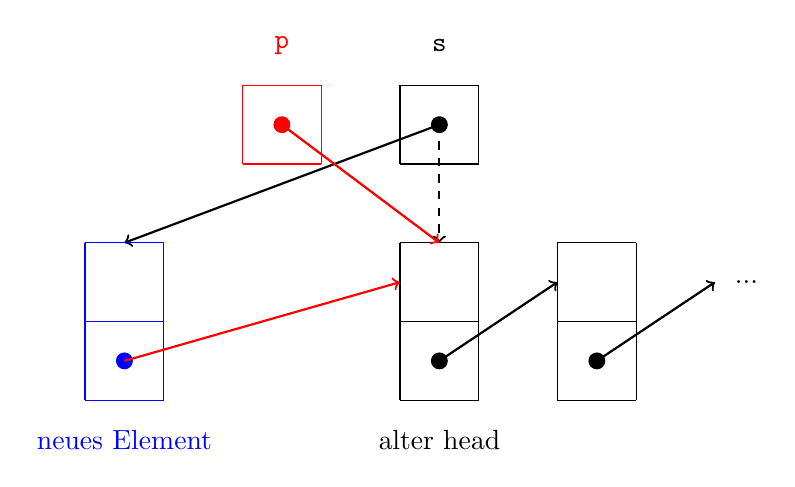
\begin{tikzpicture}
	\draw (0,-1) -- (1,-1);
	\draw (0,-2) -- (1,-2);
	\draw (0,-1) -- (0,-2);
	\draw (1,-1) -- (1,-2);
	\draw[fill=black] (0.5,-1.5) circle (0.1);
	\draw[->, thick, dashed] (0.5,-1.5) -- (0.5,-3);
	\draw[->, thick] (0.5,-1.5) -- (-3.5,-3);
	\node at (0.5,-0.5) (s) {\texttt{s}};
	
	\draw (0,-3) -- (0,-5);
	\draw (0,-3) -- (1,-3);
	\draw (1,-3) -- (1,-5);
	\draw (0,-5) -- (1,-5);
	\draw (0,-4) -- (1,-4);
	\draw[fill=black] (0.5,-4.5) circle (0.1);
	\draw[->, thick] (0.5,-4.5) -- (2,-3.5);
	\node at (0.5,-5.5) (alt) {alter head};
	
	\draw (2,-3) -- (2,-5);
	\draw (2,-3) -- (3,-3);
	\draw (3,-3) -- (3,-5);
	\draw (2,-5) -- (3,-5);
	\draw (2,-4) -- (3,-4);
	\draw[fill=black] (2.5,-4.5) circle (0.1);
	\draw[->, thick] (2.5,-4.5) -- (4,-3.5);
	\node at (4.4,-3.5) (n) {...};
	
	\draw[red] (-2,-1) -- (-1,-1);
	\draw[red] (-2,-2) -- (-1,-2);
	\draw[red] (-2,-1) -- (-2,-2);
	\draw[red] (-1,-1) -- (-1,-2);
	\draw[fill=red, red] (-1.5,-1.5) circle (0.1);
	\draw[->, thick, red] (-1.5,-1.5) -- (0.5,-3);
	\node[red] at (-1.5,-0.5) (s) {\texttt{p}};
	
	\draw[blue] (-4,-3) -- (-3,-3);
	\draw[blue] (-4,-3) -- (-4,-5);
	\draw[blue] (-3,-3) -- (-3,-5);
	\draw[blue] (-4,-4) -- (-3,-4);
	\draw[blue] (-4,-5) -- (-3,-5);
	\draw[fill=blue, blue] (-3.5,-4.5) circle (0.1);
	\draw[->, thick, red] (-3.5,-4.5) -- (0,-3.5);
	\node[blue] at (-3.5,-5.5) (neu) {neues Element};
	\end{tikzpicture}
\end{center}

Zuerst haben wir die schwarze Liste mit \texttt{s} als heap-Pointer. Für spätere Verwendung setzen wir noch den Nachfolger eines \textcolor{red}{\texttt{p}}-Pointer auf den head. Jetzt wird das \textcolor{blue}{neue Element} eingefügt und der \texttt{s}-Pointer zeigt auf den neuen head. Der Nachfolger des neuen head muss nun noch auf \textcolor{red}{\texttt{p}} zeigen, was ja auf den alten head zeigt. Schon ist das \textcolor{blue}{neue Element} eingebunden.

\subsubsection*{\texttt{pop(s,elem)}}

\begin{center}
	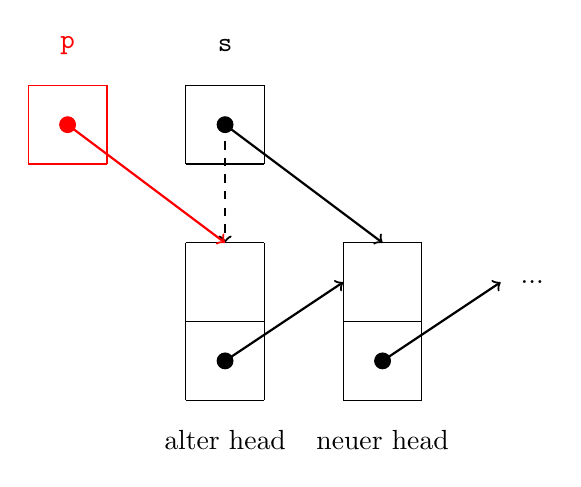
\begin{tikzpicture}
	\draw (0,-1) -- (1,-1);
	\draw (0,-2) -- (1,-2);
	\draw (0,-1) -- (0,-2);
	\draw (1,-1) -- (1,-2);
	\draw[fill=black] (0.5,-1.5) circle (0.1);
	\draw[->, thick, dashed] (0.5,-1.5) -- (0.5,-3);
	\draw[->, thick] (0.5,-1.5) -- (2.5,-3);
	\node at (0.5,-0.5) (s) {\texttt{s}};
	
	\draw (0,-3) -- (0,-5);
	\draw (0,-3) -- (1,-3);
	\draw (1,-3) -- (1,-5);
	\draw (0,-5) -- (1,-5);
	\draw (0,-4) -- (1,-4);
	\draw[fill=black] (0.5,-4.5) circle (0.1);
	\draw[->, thick] (0.5,-4.5) -- (2,-3.5);
	\node at (0.5,-5.5) (alt) {alter head};
	
	\draw (2,-3) -- (2,-5);
	\draw (2,-3) -- (3,-3);
	\draw (3,-3) -- (3,-5);
	\draw (2,-5) -- (3,-5);
	\draw (2,-4) -- (3,-4);
	\draw[fill=black] (2.5,-4.5) circle (0.1);
	\draw[->, thick] (2.5,-4.5) -- (4,-3.5);
	\node at (2.5,-5.5) (neu) {neuer head};
	\node at (4.4,-3.5) (n) {...};
	
	\draw[red] (-2,-1) -- (-1,-1);
	\draw[red] (-2,-2) -- (-1,-2);
	\draw[red] (-2,-1) -- (-2,-2);
	\draw[red] (-1,-1) -- (-1,-2);
	\draw[fill=red, red] (-1.5,-1.5) circle (0.1);
	\draw[->, thick, red] (-1.5,-1.5) -- (0.5,-3);
	\node[red] at (-1.5,-0.5) (s) {\texttt{p}};
	\end{tikzpicture}
\end{center}

Wir haben wieder die schwarze Liste mit \texttt{s}-Pointer. Um auf den alten head zugreifen zu können, benutzen wir wieder den Hilfspointer \textcolor{red}{\texttt{p}}. Den \texttt{s}-Pointer setzen wir dann auf den Nachfolger des alten heads.

\subsubsection*{\texttt{inject(t,elem)}}

Der Nachfolger des alten tails zeigt nun auf das neue Element. Dann muss nur noch der tail-Pointer angepasst werden und der Nachfolger des neuen tails muss mit \texttt{nullify} auf Null gesetzt werden.

\subsubsection*{\texttt{eject(t,elem)}}

Hier bekommen wir ein Problem! Nicht das es nicht möglich wäre das letzte Element zu löschen, aber der Vorgänger des tail-Elements kann nur gefunden werden, indem man die ganze Liste durchläuft. Das heißt die Laufzeitkomplexität dieser Operation beträgt $T(n)=\mathcal{O}(n)$. Die Dauer dieser Operation ist also von der Listenlänge abhängig!
\section{Queues}

Eine \begriff{Queue} ist eine Warteschlange und sollte mit \texttt{pop} und \texttt{inject} implementiert werden. Es ist dabei in 2 verschiedene Prinzipien zu unterscheiden:
\begin{itemize}
	\item Beim \begriff{FIFO-Prinzip} (first-in-first-out) wird das erste Element, was in die Warteschlange kommt, bearbeitet und verlässt die Warteschlange (so wie bei der Kassenschlange in der Mensa).
	\item Beim \begriff{LIFO-Prinzip} (last-in-first-out) wird das Element, was zuletzt in die Warteschlange kommt, bearbeitet (nach dem Prinzip bearbeite ich Mails: die neuste beantworte ich zuerst).
\end{itemize}

\smiley{} Professor Walter bevorzugt übrigens das LIFO-Prinzip in der Mensa. Er kommt zuletzt, hat aber als Erster sein Essen. \smiley{}

Weiterhin gibt es noch Output-resticted-queues bzw. Input-restricted-queues. Das sind deques mit \texttt{push}, \texttt{pop}, \texttt{inject}, aber ohne \texttt{eject} bzw. eine deque mit \texttt{pop} und \texttt{eject} oder \texttt{push} und \texttt{inject}.

\subsection{Grundoperationen auf einer Queue}

Eine Queue hat 4 wichtige Funktionen:
\begin{itemize}
	\item \texttt{init(Q,n)}
	\item \texttt{empty(Q)} bzw. \texttt{full(Q)}
	\item \texttt{enqueue(Q,neu)}: \texttt{inject} am tail
	\item \texttt{dequeue(Q)}: \texttt{pop} am head
\end{itemize}

Implementiert wird dies mit einem eindimensionalen Feld mit \texttt{maxlengh}, \texttt{index\_head}, \texttt{index\_tail} und \texttt{elems} (Pointer auf Feld \texttt{Q}). Hier sind die notwendigen Funktionen nur angedeutet, Details kann sich jeder selber denken.

\begin{lstlisting}
subroutine init(Q,n)
 type(queue) :: Q
 integer :: n
 
 allocate(Q(0:n-1))
 maxlengh = n
 index_head = 0
 index_tail = n-1
end subroutine init

function empty(Q)
 type(queue) :: Q
 logical :: empty
 
 empty = mod(index_tail+1,n) == index_head

end function empty

function full(Q)
type(queue) :: Q
logical :: full

 full = mod(index_tail+2,n) == index_head
 ! ein Element bleibt ungenutzt

end function full

subroutine enqueue(Q,neu)
 type(queue) :: Q
 type(element) :: neu
 
 ! ...
 index_tail = mod(index_tail+1,n)
end subroutine enqueue

subroutine dequeue(Q)
type(queue) :: Q

! ...
index_head = mod(index_head+1,n)
end subroutine dequeue
\end{lstlisting}
\section{Rechenaufwand für Grundoperationen}

\begin{tabularx}{\textwidth}{p{0.17\textwidth}|p{0.16\textwidth}p{0.16\textwidth}|p{0.17\textwidth}p{0.2\textwidth}}
	 & einfach verkettet & & doppelt verkettet & \\
	 \hline
	 Grundoperationen & linear & zyklisch & linear & zyklisch \\
	 \hline\hline
	 \texttt{access\_head} & konstant & konstant & konstant & konstant \\
	 \hline
	 \texttt{push} & konstant & konstant & konstant & konstant \\
	 \hline
	 \texttt{pop} & konstant & konstant & konstant & konstant \\
	 \hline
	 \texttt{access\_tail} [mit tail-Pointer] & $\mathcal{O}(n)$ [konstant] & konstant & $\mathcal{O}(n)$ [konstant] & konstant \\
	 \hline
	 \texttt{inject} [mit tail-Pointer] & $\mathcal{O}(n)$ [konstant] & konstant & $\mathcal{O}(n)$ [konstant] & konstant \\
	 \hline
	 \texttt{eject} [mit tail-Pointer] & $\mathcal{O}(n)$ & $\mathcal{O}(n)$ & $\mathcal{O}(n)$ [konstant] & konstant \\
	 \hline
	 \texttt{insert\_before} & $\mathcal{O}(n)$ & $\mathcal{O}(n)$ & konstant & konstant \\
	 \hline
	 \texttt{insert\_after} & konstant & konstant & konstant & konstant \\
	 \hline
	 \texttt{del\_elem} & $\mathcal{O}(n)$ & $\mathcal{O}(n)$ & konstant & konstant \\
	 \hline
	 \texttt{del\_after} & konstant & konstant & konstant & konstant \\
	 \hline
	 \texttt{trav\_forward} & konstant (pro Element) & konstant (pro Element) & konstant (pro Element) & konstant (pro Element) \\
	 \hline
	 \texttt{trav\_backward} & $\mathcal{O}(n)$ (pro Element) & $\mathcal{O}(n)$ (pro Element) & $\mathcal{O}(n)$ (pro Element) & $\mathcal{O}(n)$ (pro Element) \\
\end{tabularx}

\chapter{Bäume/Trees und Rekursion}
Ein \begriff{Baum} ist entweder leer oder besteht aus einer endlichen Menge von Knoten mit einem speziell ausgezeichneten Wurzelknoten (\begriff{root}) und einer endlichen Anzahl von Teilbäumen.

Ein Baum ist also rekursiv definiert und besitzt eine rekursive Datenstruktur. Wir brauchen deswegen rekursive Algorithmen zur Bearbeitung.

Der \begriff[Baum!]{Grad} ist die Anzahl der Verzweigungen nach unten. \\
Das \begriff[Baum!]{Level} ist die Anzahl der Ebenen, beginnend bei der Wurzel mit 0. \\
Die \begriff[Baum!]{Höhe} eines Baums ist die Weglänge zum weitest entfernten Knoten.

Wir wollen die Wechselbeziehung zwischen einer rekursiven Datenstruktur und einem rekursiven Algorithmus untersuchen. Dazu ist es notwendig zu wissen, dass man die Ausführung rekursiver Algorithmen als Baum darstellen kann, so zum Beispiel die \person{Fibonacci}-Zahlen. Sei dazu $F_n$ die $n$-te \person{Fibonacci}-Zahl:
\begin{center}
	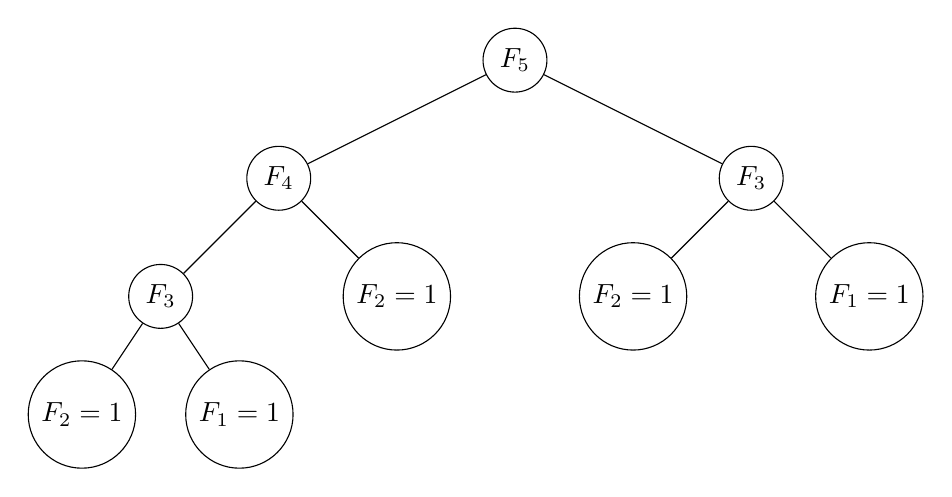
\begin{tikzpicture}[level/.style={sibling distance=60mm/#1}]
		\node[circle, draw] (root) {$F_5$}
			child {node[circle,draw] (a) {$F_4$}
				child {node[circle,draw] (b) {$F_3$}
					child {node[circle,draw] (c) {$F_2 = 1$}}
					child {node[circle,draw] (d) {$F_1 = 1$}}}
				child {node[circle,draw] (e) {$F_2 = 1$}}}
			child {node[circle,draw] (f) {$F_3$}
				child {node[circle,draw] (g) {$F_2 = 1$}}
				child {node[circle,draw] (h) {$F_1 = 1$}}};
	\end{tikzpicture}
\end{center}

Man unterscheidet dabei in die \begriff{Rechtsrekursion} und die \begriff{Linksrekursion}.
\begin{center}
	\begin{tabularx}{\textwidth}{l|l} %TODO: Tabelle bearbeiten
		\textbf{Rechtsrekursion} & \textbf{Linksrekursion} \\
		\hline
		Ein Problem $P_n$ lässt sich durch Ausführen eines Tasks $T_n$ das betrachten des Problems $P_{n-1}$ lösen. & Ein Problem $P_n$ lässt sich durch betrachten des Problems $P_{n-1}$ und anschließendes Ausführen eines Tasks $T_n$ lösen. \\
		Also lässt sich $P_n$ durch Ausführung von $T_nT_{n-1}\dots T_1T_0$ lösen. Diese Rekursion ist leicht auflösbar. Das Problem lässt sich iterativ lösen. & Also lässt sich $P_n$ durch Ausführung von $T_0T_1\dots T_{n-1}T_n$ lösen. Diese Rekursion ist nicht leicht auflösbar; sie benötigt einen Stack, da man den Speicherzustand von $T_0$ nicht aus $T_n$ vorhersagen kann.
	\end{tabularx}
\end{center}

Bei einer \begriff{allgemeinen Rekursion} sieht das Problem $P_{n,j}$  so aus.
\begin{align}
	P_{n,j} = \begin{cases}
		T_0 & n=0 \\ T_0P_{n-1,1}T_1P_{n-1,2}\dots T_{k-1}P_{n-1,k}T_k & n>0
	\end{cases} 1\le i \le k\notag
\end{align}
Auch hier genügt die Abarbeitung einem Stack!

Ein \begriff{Binärbaum} ist ein Baum mit maximalem Knotengrad 2.
\begin{itemize}
	\item maximale Anzahl an Knoten auf dem Level $l$: $2^l$
	\item maximale Anzahl Knoten auf dem gesamten Baum: $N=\sum\limits_{l=0}^h 2^l = 2^{h+1}-1$
	\item minimale Höhe eines Baums mit $N$ Knoten: $h_{min}=\lfloor\log_2 N\rfloor$
\end{itemize}

\section{Binäre Suchbäume}

Ein \begriff{binärer Suchbaum} ist ein Binärbaum, bei dem im linken Teilbaum eines Knotens nur "'kleinere'" Elemente und im rechten Teilbaum nur "'größere'" Elemente gespeichert sind. Dabei gibt es immer eine besondere Datenkomponente, die als Schlüssel (Key) dient und deren Werte eine vollständige Ordnung ermöglichen (Ordnungsrelation, typischerweise $<$).

Die elementaren Operationen auf Binärbäumen sind:
\begin{itemize}
	\item Traversieren:
	\begin{itemize}
		\item \begriff{Preorder}: $P(B)=T(B)P(B_L)P(B_R)$
		\item \begriff{Inorder}: $P(B)=P(B_L)T(B)P(B_R)$
		\item \begriff{Postorder}: $P(B)=P(B_L)P(B_R)T(B)$
		\item \begriff{Levelorder}: schichtweises Durchlaufen von oben nach unten, von links nach rechts
	\end{itemize}
	\item Einfügen und suchen: Beim Durchlaufen (Traversieren) in Inorder erhält man die in aufsteigender Schlüsselreihenfolge sortierten Elemente/Knoten(inhalte).
	\item Löschen eines Knotens mit gesuchtem Schlüsselwert im Suchbaum:
	\begin{itemize}
		\item Blatt löschen ist einfach (keine Teilbäume)
		\item Knoten hat genau einen Teilbaum: listenartige Reparatur
		\item innerer Knoten mit 2 nichtleeren Teilbäumen: 2 Möglichkeiten
		\begin{itemize}
			\item größeres Element im linken Teilbaum (des zu löschenden Knotens) suchen, dieses hat rechten Teilbaum $\Rightarrow$ diesem Knoten durch seinen linken Teilbaum ersetzen, Inhalt dieses
			(ersetzten) Elements in den „zu löschenden“ Knoten kopieren, sodann dieses größere Element (d.h. seinen Knoten) mittels 1 oder 2 löschen (Speicher freigeben!)
			\item kleines Element im rechten Teilbaum (des zu löschenden Knotens) suchen, dieses hat linken Teilbaum $\Rightarrow$ diesem Knoten durch seinen rechten Teilbaum ersetzen, Inhalt dieses (ersetzten) Elements in den „zu löschenden“ Knoten kopieren, sodann dieses kleinere Element (d.h. seinen Knoten) mittels 1 oder 2 löschen (Speicher freigeben!)
		\end{itemize}
	\end{itemize}
\end{itemize}

Ein \begriff{Sentinel} (Wachposten) ist ein Knoten, der den zu suchenden Schlüssel enthält. Alle Nullpointer eines Trees zeigen auf den Sentinel. Das sorgt dafür, dass, wenn man einen Schlüssel sucht, nach links (bei kleiner) bzw. nach rechts (bei größer) geht; ist der Wert gleich muss man nur noch schauen, ob der gefundene Wert der Sentinel ist, dann ist der gesuchte Wert nicht enthalten, andernfalls schon.

\chapter{Suchen und Sortieren}
\section{Begriffe und Definitionen}

Beim \begriff{linearen Suchen} sucht man in einem unsortierten Feld mit $n$ Elementen. Der Aufwand liegt zwischen 1 und $n$, ist also linear abhängig von der Anzahl der Elemente. $T(n)=\mathcal{O}(n)$

Beim \begriff{binären Suchen} muss das Feld schon sortiert sein. Man fragt dabei den Schlüsselwert des mittleren Elements ab und kann so den zu durchsuchenden Bereich in jedem Schritt halbieren. $T(n)=\mathcal{O}(\log_2 n)$

\begin{*anmerkung}
	Dieses Verfahren wurde im letzten Semester schon in der Aufgabe zum Zahlenraten verwendet.
\end{*anmerkung}

Man kann Sortierverfahren nach ihrem Speicherplatzbedarf unterteilen: \begriff{in-situ Sortierverfahren} vs. \begriff{externes Sortierverfahren}
%\begin{center}
%	\begin{tabularx}{\textwidth}{l|l} %TODO: Tabelle
%		\textbf{in-situ} & \textbf{extern} \\
%		\hline
%		\begin{itemize}
%			\item alle $n$ Elemente sind schon zu Beginn (in beliebiger Anordnung) im Feld gespeichert
%			\item die Elemente werden (bis auf eventuelle notwendige kurzzeitige Auslagerung eines Elements)
%			immer in diesem Feld gehalten
%			\item insbesondere wird nur eine sehr kleine Zahl zusätzlicher skalarer Varianten benötigt (und keine
%			zusätzliche Datenstruktur mit $c \cdot n$ Elementen ($0 < c < 1$))
%		\end{itemize} & 
%		\begin{itemize}
%			\item Sortierung erfolgt nicht nur im Originalfeld
%			\item benötigt typischerweise $\mathcal{O}(n)$ zusätzlichen Speicherplatz
%		\end{itemize} \\
%	\end{tabularx}
%\end{center}

Ein Sortierverfahren ist \begriff{stabil}, wenn es die relative Ordnung von Elementen mit dem selben Schlüsselwert nicht ändert.

Ein \begriff{Mikroschritt} bzw. eine \begriff{Elementaroperation} besteht in der Regel aus einem Vergleich von 2 Schlüsselwerten und einer Kopier- oder Tauschoperation. Ein \begriff{Makroschritt} bzw. \begriff{Durchlauf} besteht aus $\mathcal{O}(n)$ Mikroschritten, zum Beispiel der Durchlauf durch alle noch zu sortierenden Elemente.

Die Zeitkomplexität von Algorithmen $T(n)$ wird mit den \person{Landau}-Operatoren angegeben:
\begin{itemize}
	\item $\mathcal{O}(g(n))=\{f(n):\exists c>0, n_0\in\natur_0\mid 0\le f(n)\le c\cdot g(n)\quad\forall n\ge n_0\}$ (Obergrenze)
	\item $\Omega(g(n)) = \{f(n):\exists c>0, n_0\in\natur_0\mid 0\le c\cdot g(n)\le f(n)\quad\forall n\ge n_0\}$ (Untergrenze)
	\item $\Theta(g(n)) = \{f(n):\exists c_1,c_2>0,n_0\in\natur_0\mid 0\le c_1\cdot g(n)\le f(n)\le c_2\cdot g(n)\quad\forall n\ge n_0\}$ (Sandwich)
\end{itemize}

Also gilt: $T(n) = \mathcal{O}(n^2) = \mathcal{O}(n^2\cdot\log n) = \mathcal{O}(n^2\cdot\sqrt{n}) = \mathcal{O}(n^3) = \dots = \mathcal{O}(2^n) = \mathcal{O}(n^n)$.

\begin{*anmerkung}
	Die Schreibweise kann ziemlich verwirren; es hilft sich $\mathcal{O}(n^2)$ als Menge vorzustellen, die alle Funktionen enthält, die maximal so schnell wie $n^2$ wachsen. Die Schreibweise $\mathcal{O}(n^2)=\mathcal{O}(n^2\cdot\log n)$ bedeutet dann nicht, dass diese Mengen gleich sind, sondern dass die eine Menge in der anderen enthalten ist: Es gilt also $\mathcal{O}(n^2)\in\mathcal{O}(n^2\cdot\log n)$, denn $x^2 \le x^2\cdot\log x$ für alle $x$.
\end{*anmerkung}

Sortieralgorithmen bekommen in der Regel 3 Komplexitätsangaben:
\begin{itemize}
	\item \begriff{worst case}: $\mathcal{O}(\dots)$ oder $\Theta(\dots)$
	\item \begriff{average case}: $\mathcal{O}(\dots)$, $\Omega(\dots)$ oder $\Theta(\dots)$
	\item \begriff{best case}: $\Omega(\dots)$
\end{itemize}

Im folgenden wird die \textbf{allgemeine Annahme} gelten: Sortiert wird immer in einem eindimensionalen Feld $A$ mit Indexmenge $I$ mit der Relation $\le$ bezüglich des Schlüssels in aufsteigender Reihenfolge.

Es gibt mindestens 2 Möglichkeiten, Datenelemente im Feld $A$ zu sortieren:
\begin{enumerate}
	\item \begriff{direktes Sortieren}: Bewegen der Datenelemente inklusive key
	\item \begriff{indirektes Sortieren}: Erzeugen einer Sortierpermutation $\sigma$ der Indizes, wobei nur die Indizes in einem eigenen Feld und nicht die Datenelemente bewegt werden
\end{enumerate}
Im sortierten Zustand gilt für alle $i,j\in I$:
\begin{itemize}
	\item direktes Sortieren: $i < j \Rightarrow A(i) \le A(j)$
	\item indirektes Sortieren: $i < j \Rightarrow A(\sigma(i)) \le A(\sigma(j))$
\end{itemize}

Eine \begriff{Sortierpermutation} $\sigma$ einer Liste $A$ auf einer Indexmenge $I=\{1,\dots,n\}$ ist eine Permutation von $I$, das heißt $\{\sigma(1),\dots,\sigma(n)\}$ mit $\sigma(i)\neq\sigma(j)$ für $i\neq j$.
\section{3 einfache Sortieralgorithmen}

\begin{center}
	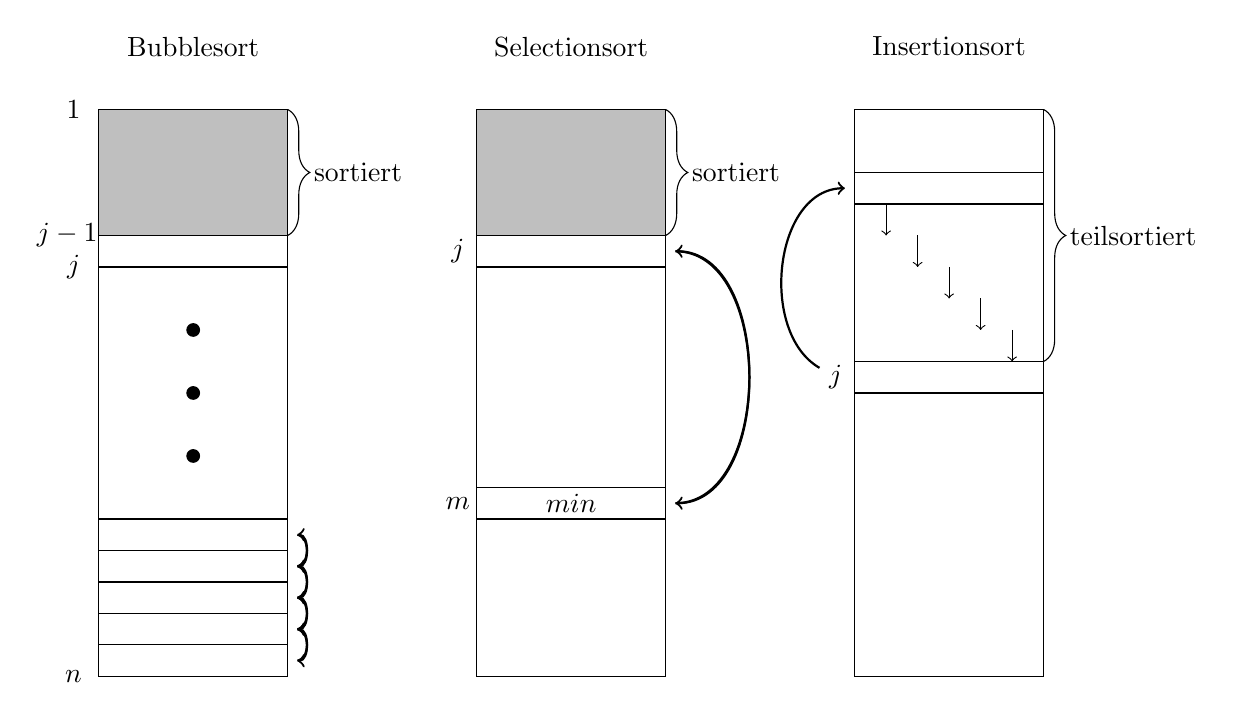
\begin{tikzpicture}[scale=0.8]
	\node at (1.5,1) (bubble) {Bubblesort};
	\draw (0,0) rectangle (3,-9);
	\draw[fill=lightgray] (0,0) rectangle (3,-2);
	\draw[decorate,decoration={brace,amplitude=8pt}] (3,0) -- (3,-2) node[midway, right, xshift=6pt]{sortiert};
	\draw (0,-2.5) -- (3,-2.5);
	\draw[fill=black] (1.5,-3.5) circle (0.1);
	\draw[fill=black] (1.5,-4.5) circle (0.1);
	\draw[fill=black] (1.5,-5.5) circle (0.1);
	\draw (0,-6.5) -- (3,-6.5);
	\draw (0,-7) -- (3,-7);
	\draw (0,-7.5) -- (3,-7.5);
	\draw (0,-8) -- (3,-8);
	\draw (0,-8.5) -- (3,-8.5);
	
	\node at (-0.4,0) (1) {1};
	\node at (-0.5,-2) (j-1) {$j-1$};
	\node at (-0.4,-2.5) (j) {$j$};
	\node at (-0.4,-9) (n) {$n$};
	
	\node at (3,-6.75) (a) {};
	\node at (3,-7.25) (b) {};
	\node at (3,-7.75) (c) {};
	\node at (3,-8.25) (d) {};
	\node at (3,-8.75) (e) {};
	\draw[->, thick] (a) to [out=0, in=0] (b);
	\draw[->, thick] (b) to [out=0, in=0] (c);
	\draw[->, thick] (c) to [out=0, in=0] (d);
	\draw[->, thick] (d) to [out=0, in=0] (e);
	\draw[->, thick] (e) to [out=0, in=0] (d);
	\draw[->, thick] (d) to [out=0, in=0] (c);
	\draw[->, thick] (c) to [out=0, in=0] (b);
	\draw[->, thick] (b) to [out=0, in=0] (a);
	
	\node at (7.5,1) (selection) {Selectionsort};
	\draw (6,0) rectangle (9,-9);
	\draw[fill=lightgray] (6,0) rectangle (9,-2);
	\draw[decorate,decoration={brace,amplitude=8pt}] (9,0) -- (9,-2) node[midway, right, xshift=6pt]{sortiert};
	\draw (6,-2.5) -- (9,-2.5);
	\node at (5.7,-2.25) (j) {$j$};
	\draw (6,-6.5) -- (9,-6.5);
	\node at (5.7,-6.25) (m) {$m$};
	\draw (6,-6) -- (9,-6);
	\node at (7.5,-6.25) (min) {$min$};
	
	\node at (9,-2.25) (g) {};
	\node at (9,-6.25) (h) {};
	\draw[->,thick] (h) to [out=0, in=0] (g);
	\draw[->,thick] (g) to [out=0, in=0] (h);
	
	\node at (13.5,1) (insert) {Insertionsort};
	\draw (12,0) rectangle (15,-9);
	\draw[decorate,decoration={brace,amplitude=8pt}] (15,0) -- (15,-4) node[midway, right, xshift=6pt]{teilsortiert};
	\draw (12,-4.5) -- (15,-4.5);
	\node at (11.7,-4.25) (j) {$j$};
	\draw (12,-4) -- (15,-4);
	\draw (12,-1) -- (15,-1);
	\draw (12,-1.5) -- (15,-1.5);
	\node at (12,-1.25) (k) {};
	\draw[->,thick] (j) to [out=150, in=180] (k);
	
	\draw[->] (12.5,-1.5) -- (12.5,-2);
	\draw[->] (13,-2) -- (13,-2.5);
	\draw[->] (13.5,-2.5) -- (13.5,-3);
	\draw[->] (14,-3) -- (14,-3.5);
	\draw[->] (14.5,-3.5) -- (14.5,-4);
	\end{tikzpicture}
\end{center}

\begin{tabular}{p{0.2\textwidth}|p{0.35\textwidth}|p{0.35\textwidth}}
	\cellcolor{lightgray}\textbf{Sortierverfahren} & \cellcolor{lightgray}\textbf{Anzahl Vergleiche} & \cellcolor{lightgray}\textbf{Anzahl Kopier-/Tauschoperationen} \\
	\hline
	\textbf{Bubblesort} & $\sum\limits_{j=1}^{n-1}(n-j) = \sum\limits_{j=1}^{n-1}\frac{n(n-1)}{2} = \mathcal{O}(n^2) = \Omega(n)$ & $\le\frac{1}{2}n(n-1)=\mathcal{O}(n^2)$ Tauschoperationen \\
	\hline
	\textbf{Selectionsort} & $\sum\limits_{j=1}^{n-1}\frac{n(n-1)}{2}=\Theta(n^2)$ & $\le n-1=\mathcal{O}(n)$ Tauschoperationen \\
	\hline
	\textbf{Insertionsort} & $\sum\limits_{j=1}^{n-1} j=\frac{n(n-1)}{2}=\mathcal{O}(n^2)$ & $\le\sum\limits_{j=1}^{n-1} j=\frac{n(n-1)}{2}=\mathcal{O}(n^2)$ \\
	mit binärer Suche im teilsortierten Teil & $\sum\limits_{j=1}^{n-1}\log_2 j=\mathcal{O}(n\log_2 n)$ & hier bleibt alles gleich \\
\end{tabular}

Allgemein kann man also sagen:
\begin{itemize}
	\item best case: 0 Bewegungen/Kopier- und Tauschvorgänge, $\Omega(n)$ Vergleiche
	\item worst case: $\mathcal{O}(n^2)$ Vergleiche und Kopier-/Tauschoperationen
\end{itemize}

\begin{tabularx}{\textwidth}{p{0.2\textwidth}|p{0.35\textwidth}|X}
	\cellcolor{lightgray} & \cellcolor{lightgray}\textbf{Vergleiche} & \cellcolor{lightgray}\textbf{Tauschoperationen} \\
	\hline
	\textbf{Bubblesort}, \textcolor{red}{stabil} & $\mathcal{O}(n^2)$ & $\mathcal{O}(n^2)$ \\
	\hline
	\textbf{Selectionsort}, \textcolor{red}{nicht stabil} & $\mathcal{O}(n^2)$ & $\mathcal{O}(n)$ \\
	\hline
	\textbf{Insertionsort}, \textcolor{red}{stabil} & ohne binäre Suche: $\mathcal{O}(n^2)$, mit binärer Suche: $\mathcal{O}(n\log_2 n)$ & $\mathcal{O}(n^2)$
\end{tabularx}
$\Rightarrow T(n)=\mathcal{O}(n^2)$ für alle 3 einfachen Sortierverfahren

\begin{proposition}
	Sortierverfahren, die auf dem Schlüsselvergleich ($<$) von jeweils 2 Elementen (und einer eventuell notwendigen Tauschoperation) beruhen, benötigen im worst case mindestens $\Omega(n\log_2 n)$ Vergleiche.
\end{proposition}
\begin{proof}
	binärer Entscheidungsbaum der Höhe $h$ zum Sortieren von $n$ Elementen, da jeder Schlüsselwertvergleich eine binäre Entscheidung liefert. Es gibt $n!$ Permutationen der $n$ verschiedenen Schlüsselwerte, also $n!$ verschiedene Sortierfolgen, das heißt $n!$ Entscheidungspfade. $\Rightarrow$ binärer Entscheidungsbaum benötigt mindestens $n!$ Blätter, um alle Anfangszustände in den einen Sortierten zu überführen. Ein Binärbaum der Höhe $h$ hat $\le 2^h$ Blätter. Also muss gelten:
	\begin{align}
		n! &\le 2^h \notag \\
		h &\ge \log_2(n!) \notag \\
		\text{Stirling:} \quad n! &= \sqrt{2\pi n}\cdot \left(\frac{n}{e}\right)^n\cdot \left(1+\mathcal{O}\left(\frac{1}{n}\right) \right) \notag \\
		n! &> \left(\frac{n}{e}\right)^n \notag \\
		h &\ge \log_2 \left( \frac{n}{e}\right)^n=n(\log_2 n-\log_2 e) \notag \\
		&= \Theta(n\log_2 n) \notag
	\end{align}
	$\Rightarrow$ mindestens $\Omega(n\log_2 n)$ Vergleiche im worst case
\end{proof}
\section{Quicksort}

Der Quicksort ist ein rekursiver Algorithmus zum Sortieren einer Liste $L$ im Indexbereich $a:e$. Erfunden wurde dieser von \person{Sir Charles Antony Richard Hoare}. Der Algorithmus läuft wie folgt ab:
\begin{enumerate}
	\item Wähle beliebiges Element aus $L$, dieses habe den key $W$ (sogenanntes \begriff{Pivotelement}). Ideal wäre, wenn $W$ der Median aller keys wäre. Der schlechteste Fall wäre, wenn $W$ ein Extremum wäre.
	\item Bilde Partition $L_L\mid L_R$ der Liste $L$ mit:
	\begin{itemize}
		\item alle Elemente von $L_L$ haben keys $\le W$
		\item alle Elemente von $L_R$ haben keys $\ge W$
	\end{itemize}
	\item Sortieren der beiden Listen mittels rekursivem Aufruf von Quicksort
\end{enumerate}

Als Quellcode sieht Quicksort dann so aus:
\begin{lstlisting}
recursive subroutine QsortC(A)
 real, intent(in out), dimension(:) :: A
 integer :: iq

 if(size(A) > 1) then
  call Partition(A, iq)
  call QsortC(A(:iq-1))
  call QsortC(A(iq:))
 endif
end subroutine QsortC

subroutine Partition(A, marker)
 real, intent(inout), dimension(:) :: A
 integer, intent(out) :: marker
 integer :: i, j
 real :: temp
 real :: x      ! pivot point

 x = A(1)
 i= 0
 j= size(A) + 1

 do
  j = j-1
  do
   if (A(j) <= x) exit
   j = j-1
  end do
  
  i = i+1
  
  do
   if (A(i) >= x) exit
   i = i+1
  end do
  
  if (i < j) then ! exchange A(i) and A(j)
   temp = A(i)
   A(i) = A(j)
   A(j) = temp
  elseif (i == j) then
   marker = i+1
   return
  else
   marker = i
   return
  endif
 end do
end subroutine Partition
\end{lstlisting}

Im worst case, das heißt das Pivotelement ist ein Extremum, wird immer nur 1 Element abgespalten. Dann hat Quicksort die Komplexität $T(n)=\mathcal{O}(n^2)$. Im average case gilt: $T(n)=\mathcal{O}(n\log_2 n)$ und im best case hat Quicksort die Komplexität $T(n)=\Omega(n\log_2 n)$.

Zuletzt noch ein Blick auf die Eigenschaften:
\begin{itemize}
	\item in situ
	\item nicht stabil
	\item hat nur sehr einfache Operationen
	\item für große $n$ sehr schnell
	\item pro Durchlauf $\mathcal{O}(n)$
	\item für kleine $n$ eher schlecht
\end{itemize}
\section{Mergesort}

\subsection{2-Wege-Mergesort}

Den Mergesort-Algorithmus gibt es in 2 Varianten: rekursiv und iterativ. Schauen wir uns zuerst die rekursive Variante an:
\begin{enumerate}
	\item falls $L$ leer oder nur 1 Element enthält $\to$ ok, return
	\item divide: Teile $L$ in 2 möglichst gleich lange Teillisten $L_1$ und $L_2$ und mache darauf rekursive Aufrufe \texttt{Mergesort(L\_1)} und \texttt{Mergesort(L\_2)}.
	\item conquer: Merge von $L_1$ und $L_2$
\end{enumerate}

\begin{lstlisting}
! kann nur 10 Elemente sortieren, kann man aber anpassen

subroutine _merge(lst, a, middle, b)
 integer a
 integer b
 integer middle
 integer lst(10)
 integer tmp(10)
 integer ai
 integer bi
 integer ti
 integer x
 ai = a
 bi = middle
 ti = a

 do while ((ai < middle) .or. (bi < b))
  if (ai == middle) then
   tmp(ti+1) = lst(bi+1)
   bi = bi + 1
  else if (bi == b) then
   tmp(ti+1) = lst(ai+1)
   ai = ai + 1
  else if (lst(ai+1) < lst(bi+1)) then
   tmp(ti+1) = lst(ai+1)
   ai = ai + 1
  else
   tmp(ti+1) = lst(bi+1)
   bi = bi + 1
  end if
  
  ti = ti + 1
 end do
 do x = a, b - 1
  lst(x + 1) = tmp(x + 1)
 end do
end subroutine _merge

recursive subroutine mergesort(lst, a, b)
 integer a
 integer b
 integer lst(10)
 integer diff
 diff = b - a
 
 if (diff < 2) then
  return
 else
  diff = diff / 2
  call mergesort(lst, a, a + diff)
  call mergesort(lst, a + diff, b)
  call _merge(lst, a, a + diff, b)
 endif
end subroutine mergesort
\end{lstlisting}

Mergesort ist nicht in situ. $T(n)=\mathcal{O}(n\log_2 n)$. All Lese- und Schreiboperationen sind streng sequenziell.

Die iterative Variante verläuft ähnlich, verwendet aber 4 Listen $L_1$, $L_2$, $L_3$ und $L_4$.
\begin{enumerate}
	\item Init: Teile $L$ in 2 möglichst gleich große Teillisten $L_1$ und $L_2$
	\item Erzeuge 2 Listen sortierter Paare, $L_3$ und $L_4$, indem positionell sich entsprechende Elemente von $L_1$ und $L_2$ jeweils zu einem sortierten Paar gemacht werden und in die zuletzt nicht benutzte Liste $L_3$ bzw. $L_4$ (immer abwechselnd) geschrieben werden
	\item Erzeuge 2 Listen sortierter Quadrupel in $L_1$ und $L_2$
	\item Erzeuge 2 Listen sortierter Oktupel in $L_3$ und $L_4$
	\item ...
\end{enumerate}

Die Komplexität ist auch hier $T(n)=\mathcal{O}(n\log_2 n)$, tatsächlich ist die Zeit $T(n)=\Theta(n\log_2 n)$ immer die selbe, egal ob best- oder worst case.

\subsection{$k$-Wege-Mergesort}

Hier existiert nur eine rekursive Variante, in der die Liste in $k$ Teillisten aufgeteilt wird. Man kann aber auch mit $k$ Input-Listen und $k$ Output-Listen arbeiten. Noch einige Bemerkungen:
\begin{itemize}
	\item Für den Mergeschritt wird ein $k$-elementiger Vektor von Schlüsselwerten benötigt, um die jeweils aktuellen Kopfelemente der $k$ zu verschmelzenden Listen sortiert zu speichern.
	\item Die Anzahl der Durchläufe reduziert sich gegenüber dem 2-Wege-Mergesort von $\lceil\log_2 n\rceil$ auf $\lceil\log_k n\rceil$, also um den Faktor $\frac{1}{\log_2 k}=\log_k 2$, zum Beispiel bei $k=1024=2^{10}$ Teillisten auf $\frac{1}{10}$.
\end{itemize}

\begin{tabularx}{\textwidth}{X|p{0.13\textwidth}p{0.1\textwidth}p{0.09\textwidth}p{0.1\textwidth}p{0.08\textwidth}|p{0.17\textwidth}}
	\rowcolor{lightgray} \textbf{Markoschritt} & \textbf{produziert} & \textbf{$k$-Tupel sortieren} & \textbf{Anzahl Elemente} & \textbf{Aufwand Insertion-Schritt} & \textbf{Anzahl Tupel} & \textbf{Aufwand} \\
	\hline
	\textbf{1} & $k$-Tupel: $\mathcal{O}($ & $(k\log_2 k+$ & $0\cdot$ & $\mathcal{O}(k))$ & $\cdot\frac{n}{k})$ & $\mathcal{O}(n\log_2 k)$ \\
	\textbf{2} & $k^2$-Tupel: $\mathcal{O}($ & $(k\log_2 k+$ & $k(k-1)\cdot$ & $\mathcal{O}(k))$ & $\cdot\frac{n}{k^2})$ & $\mathcal{O}(nk)$ \\
	\textbf{3} & $k^3$-Tupel: $\mathcal{O}($ & $(k\log_2 k+$ & $(k^3-k)\cdot$ & $\mathcal{O}(k))$ & $\cdot\frac{n}{k^3})$ & $\mathcal{O}(nk)$ \\
	\vdots & \vdots & \vdots & \vdots & \vdots & \vdots & \vdots \\
	\hline
	&&&&&& $\Sigma = \mathcal{O}(kn\log_2 n)$ \\
\end{tabularx}
\section{Heapsort}

\begin{*anmerkung}
	Das folgende Kapitel ist ziemlich durcheinander; ich glaube Prof. Walter wusste selber nicht so richtig, was er wollte. Es empfiehlt sich ein Youtube-Tutorial anzuschauen, um zu verstehen, wie Heapsort funktioniert.
\end{*anmerkung}

Ein binärer \begriff{Heap} ist ein vollständiger Binärbaum mit der sogenannten \begriff{Heap-Eigenschaft}: Ein vollständiger Binärbaum hat alle Schichten ab der Wurzel voll besetzt bis auf eventuell die letzte, die von links nach rechts bis zum letzten Knoten besetzt ist. Die Vollständigkeit garantiert, dass ein eindimensionales Feld \texttt{A(1:n)} mit den Elementen des Heaps in Levelorder abgespeichert keine Lücken aufweist. Außerdem gilt:
\begin{lstlisting}
! Index des linken Kindknotens des Knotens mit Index i
Left(i) = 2*i
! Index des rechten Kindknotens des Knotens mit Index i
Right(i) = 2*i+1
! i/2 ist Index des Elternknotens
Parent(i) = i/2
\end{lstlisting}
$\Rightarrow$ Dualität eines Heaps und eines vollständigen Binärbaums; außerdem Höhe $h=\Theta(\log_2 n)$.

\textbf{Zusätzliche Heap-Eigenschaft}: $A_{\texttt{Parent(i)}} \ge A_\texttt{i}$, das heißt Schlüsselwert des Elternelements $\ge$ Schlüsselwerte der beiden Kindknoten.

Um aus einem Feld $A$ einen Heap zu machen, brauchen wir eine Subroutine \texttt{Heapify}. Die folgenden Quelltexte sind nur ein Konzept, soweit ich weiß, muss man sie nirgendwo reproduzieren.
\begin{lstlisting}
n = size(A)

subroutine Heapify(A,i)
 r = Right(i)
 l = Left(i)
 maxix = i
 
 if(l <= size .and. A_l > A_i) then
  maxix = l
 end if
 if(r <= size .and. A_r > A_maxix) then
  maxix = r
 end if
 if(maxix /= i) then
  tausche(A_i,A_maxix)
  Heapify(A,maxix)
 end if
end subroutine Heapify
\end{lstlisting}

Der Zeitaufwand für \texttt{Heapify(A,i)} ist proportional zur Höhe des Knotens mit Index $i$: \\
$T_\texttt{Heapify}=\mathcal{O}(h)$ mit $h=$\texttt{height(A,i)}$=\mathcal{O}(\log_2 n)$.

\begin{lstlisting}
subroutine BuildHeap(A)
 size = n
 
 do i = n/2, 1, -1
  Heapify(A,i)
 end do
end subroutine BuildHeap
\end{lstlisting}

Versuchen wir uns an einer Komplexitätsanalyse: $T_\texttt{BuildHeap}(n) = \mathcal{O}\left(\frac{n}{2}\log_2 n\right) = \mathcal{O}(n\log_2 n)$. Eine bessere Analyse bekommen wir, wenn die Höhe der Knoten betrachten: In einem Heap haben höchstens $\left\lceil\frac{n}{2^{n+1}}\right\rceil$ Knoten die Höhe $h$. \\
$\Rightarrow$ Gesamtaufwand für \texttt{BuildHeap}:
\begin{align}
	\sum_{h=0}^{\lfloor\log_2 n\rfloor}\left\lceil\frac{n}{2^{h+1}}\right\rceil\cdot\mathcal{O}(h) &= \mathcal{O}\left( n\cdot\sum_{h=0}^{\lfloor\log_2 n\rfloor} h\cdot \left( \frac{1}{2}\right)^h\right) \notag \\
	\sum_{k=0}^n x^k &= \frac{x^{n+1}-1}{x-1} \notag \\
	0<x<1: \quad \sum_{k=0}^\infty k\cdot x^k &= \frac{1}{1-x}=(1-x)^{-1} \notag \\
	\text{Differenzieren} \quad \sum_{k=1}^\infty k\cdot x^{k-1}&=\frac{1}{(1-x)^2} \notag \\
	x=\frac{1}{2}:\quad \sum_{k=1}^\infty k\cdot \left(\frac{1}{2}\right) &= \frac{\frac{1}{2}}{\left( \frac{1}{2}\right)^2}=2 \notag \\
	\Rightarrow T(n) &= \mathcal{O}(n)\notag
\end{align}

\begin{lstlisting}
subroutine Heapsort(A)
BuildHeap(A) ! O(n)
 do i=1, 2, -1 ! n-1 Iterationen
  tausche(A_i,A_1) ! O(1)
  size = size - 1 ! O(1)
  Heapify(A,1) ! O(log n)
 end do
end subroutine Heapsort
\end{lstlisting}
$\Rightarrow T_\texttt{Heapsort}(n)=\mathcal{O}(n)+(n-1)\mathcal{O}(\log_2 n)=\mathcal{O}(n\log_2 n)$
\section{Priority Queue}

Eine Priority Queue ist eine Art von Warteschlange, die nicht nach dem FIFO-Prinzip arbeitet, sondern die Elemente entsprechend ihrer Priorität (ein spezieller Key) behandelt. Implementiert wird dies durch einen Heap in einem eindimensionalen Feld.

\begin{*anmerkung}
	Die Grundoperationen einer Priority Queue und deren Komplexitäten werden gerne in Klausuren abgefragt.
\end{*anmerkung}

Die Grundoperationen einer Priority Queue sind wie folgt:
\begin{itemize}
	\item \texttt{init(A)} $\to$ initiiert eine leeres Feld \texttt{A}
	\item \texttt{empty(A)} $\to$ ist Feld leer?
	\item \texttt{HeapInsert(A,key)} $\to$ neues Element mit \texttt{key} einfügen in \texttt{A}
	\item \texttt{HeapExtractMax(A,key)} $\to$ key des Wurzelknotens wird in 2. Parameter (oder als Funktionswert) zurückgegeben und dieses Element aus \texttt{A} herausgenommen
	\item \texttt{HeapUpdate(A,key,max)} $\to$ Kombination aus \texttt{HeapExtractMax} und \texttt{HeapInsert}: liefert in \texttt{max} den Key der Wurzel und ersetzt diesen Wert durch \texttt{key}
	\item \texttt{Maximum(A)} $\to$ Funktion, liefert den key der Wurzel
\end{itemize}

\begin{lstlisting}
subroutine HeapExtractMax(A, max)
 if (size <= 0) error("empty heap")
 
 max = A_1
 A_1 = A_size
 size = size - 1
 Heapify(A,1)
end subroutine HeapExtractMax
\end{lstlisting}
$\Rightarrow T(n)=\mathcal{O}(\log_2 n)$

\begin{lstlisting}
subroutine HeapUpdate(A, key, max)
 if (size <= 0) error("empty heap")
 
 max = A_1
 A_1 = key
 Heapify(A,1)
end subroutine HeapUpdate
\end{lstlisting}
$\Rightarrow T(n)=\mathcal{O}(\log_2 n)$

\begin{lstlisting}
subroutine HeapInsert(A, key)
 size = size + 1
 i = size
 
 do while (i > 1 .and. A_Parent(i) < key)
  A_i = A_Parent(i)
  i = Parent(i)
 end do
 A_i = key
end subroutine HeapInsert
\end{lstlisting}
$\Rightarrow T(n)=\mathcal{O}(\log_2 n)$

\begin{lstlisting}
subroutine BuildHeapNew(A)
 size = 1
 
 do i = 2, n
  HeapInsert(A,A_i)
 end do
end subroutine BuildHeapNew
\end{lstlisting}
$\Rightarrow T(n)=\mathcal{O}(\log_2 n)$
\section{Counting Sort}

Der Counting Sort-Algorithmus ist dann besonders gut, wenn alle möglichen Schlüsselwerte aus der Menge $S=\{0,1,2,...,k-1\}$ kommen. Wenn $k=\mathcal{O}(n)$, dann können wir mit Counting Sort in der Zeit $T(n)=\mathcal{O}(n)$ sortieren. Benötigt werden 3 eindimensionale Felder:
\begin{itemize}
	\item \texttt{A(1:n)} Originaldaten/-schlüsselwerte
	\item \texttt{B(1:n)} für sortierte Werte
	\item \texttt{C(0:k-1)} Feld von Zählern
\end{itemize}
Der Algorithmus zählt, wie oft jeder Wert in der Eingabe vorkommt. Diese Anzahlen speichert er in einem zusätzlichen Array mit $k$ Feldern ab. Mit Hilfe dieses Arrays wird anschließend für jeden Schlüsselwert die Zielposition in der Ausgabe berechnet.

\begin{*anmerkung}
	Der Counting Sort ist also dann besonders gut, wenn man alle Einwohner Deutschlands ($\sim$ 81 Millionen) nach ihrem Alter ($S=\{0,...,150\}$) sortieren möchte. \\
	Der Counting Sort eignet sich nicht dafür die Studenten der PROG-Vorlesung ($\sim$ 30 \smiley{}) nach ihrem Nachnamen (40 Zeichen $\Rightarrow S=\{0,...,26^{40}\}$) zu sortieren.
\end{*anmerkung}

\begin{lstlisting}
subroutine counting_sort_a(array)
 integer, dimension(:), intent(inout) :: array

 call counting_sort_mm(array, minval(array), maxval(array))
end subroutine counting_sort_a

subroutine counting_sort_mm(array, tmin, tmax)
 integer, dimension(:), intent(inout) :: array
 integer, intent(in) :: tmin, tmax
 integer, dimension(tmin:tmax) :: cnt
 integer :: i, z

 cnt = 0 ! Initialize to zero to prevent false counts
 
 forall (i=1:z)  
  ! Not sure that this gives any benefit over a DO loop.
  cnt(array(i)) = cnt(array(i))+1
 end forall
 
 ! ok - cnt contains the frequency of every value
 ! let's unwind them into the original array
 
 z = 1
 do i = tmin, tmax
  do while ( cnt(i) > 0 )
   array(z) = i
   z = z + 1
   cnt(i) = cnt(i) - 1
  end do
 end do
end subroutine counting_sort_mm
\end{lstlisting}
\section{Radix-/Distribution Sort}

Wenn wir annehmen, dass der Schlüssel $z$ sich als Zahl mit $d$ Ziffern zur Basis $k$ darstellen lässt, also $z=[z_{d-1}z_{d-2}...z_1z_0]_k=\sum_{i=0}^{d-1}z_ik^i$, dann lässt sich mit Radix-/Distribution Sort in $T(n)=\Theta(d(n+k))$ sortieren. Falls $k=\mathcal{O}(n)$, dann $T(n)=\Theta(dn)$ und falls $d$ relativ klein ist, dann $T(n)=\Theta(n)$.

\begin{lstlisting}
subroutine RadixSort (A,B,k)
 do i = 0, d-1
  CountingSort(A,B,i,k)
 end do
end subroutine RadixSort
\end{lstlisting}

\chapter{Rekursion, Iteration, Komplexität}
\section{Beispiele}

Neben der Zeitkomplexität $T(n)$ werden wir uns nun auch mit der Speicherkomplexität $S(n)$ beschäftigen.

\begin{*anmerkung}
	Es nicht unbedingt entscheidend, alle Komplexitäten auswendig zu lernen. Vielmehr sollte man wissen, wie die Algorithmen dahinter arbeiten und sich so die Komplexitäten herleiten.
\end{*anmerkung}

\subsection{Fakultät}
\begin{lstlisting}
recursive function fac (n) result (res) 
 integer :: n
 integer :: res
 
 if (n == 1) then 
  res = 1
 else
  res = n*fac(n-1)
 end if
end function fac
\end{lstlisting}
$\Rightarrow T(n) = \Theta(n)$, $S(n)=\Theta(n)$

\begin{lstlisting}
function fac_iterativ (n)
 integer :: n, fac_iterativ, i
 
 fac_iterativ = 1
 
 do i = 1, n
  fac_iterativ = fac_iterativ * i
 end do
end function fac_iterativ
\end{lstlisting}
$\Rightarrow T(n)=\Theta(n)$, $S(n)=\Theta(1)$

\subsection{Reverse String}
\begin{lstlisting}
recursive function reverse (string) result (res)
 character (*), intent (in) :: string
 character (len (string)) :: res

 if (len (string) == 0) then
  res = ""
 else
  res = string(len(string):)//reverse(string(:len(string)-1))
 end if
end function reverse
\end{lstlisting}
$\Rightarrow T(n) = \Theta(n)$, $S(n)=\Theta(n)$

\begin{lstlisting}
program reverse_iterativ
 character(80) :: str = "This is a string"
 character :: temp
 integer :: i, length

 write(*,*) str
 length = len_trim(str) 
 ! Ignores trailing blanks. 
 ! Use len(str) to reverse those as well
 
 do i = 1, length/2
  temp = str(i:i)
  str(i:i) = str(length+1-i:length+1-i)
  str(length+1-i:length+1-i) = temp
 end do
 
 write(*,*) str
end program reverse_iterativ
\end{lstlisting}
$\Rightarrow T(n) = \Theta(n)$, $S(n)=\Theta(n)$

\subsection{Primzahl}

Um zu überprüfen, ob eine Zahl eine Primzahl ist, muss man immer bis zur Wurzel dieser Zahl auf Teiler prüfen. Egal ob man das rekursiv oder iterativ macht, $T(n)=\mathcal{O}(\sqrt{n})$. Die Speicherkomplexität ist beim rekursiven schwer vorher zu sagen, beim iterativen Algorithmus ist die $S(n)=\Theta(1)$.

\subsection{\person{Fibinacci}-Zahlen}
\begin{lstlisting}
recursive function fibR(n) result(fib)
 integer, intent(in) :: n
 integer :: fib

 select case (n)
  case (:0); fib = 0
  case (1); fib = 1
  case default; fib = fibR(n-1) + fibR(n-2)
 end select
end function fibR
\end{lstlisting}
$\Rightarrow T(n) = \Theta(\Phi^n)$, $S(n)=\mathcal{O}(2^n)$

\begin{lstlisting}
function fibI(n)
 integer, intent(in) :: n
 integer, parameter :: fib0 = 0, fib1 = 1
 integer :: fibI, back1, back2, i

 select case (n)
  case (:0); fibI = fib0
  case (1); fibI = fib1
  case default
   fibI = fib1
   back1 = fib0
   do i = 2, n
    back2 = back1
    back1 = fibI
    fibI   = back1 + back2
   end do
 end select
end function fibI
\end{lstlisting}
$\Rightarrow T(n) = \Theta(n)$, $S(n)=\Theta(1)$

Man kann die $n$-te \person{Fibonacci}-Zahl $F_n$ auch direkt berechnen:
\begin{align}
	F_n = \frac{\Phi^n-(1-\Phi^n)}{\sqrt{5}}\notag
\end{align}
Hier wird eine ganzzahlige Potenzierung benötigt, die eine Komplexität von $T(n)=\Theta(\log_2 n)$ hat.

\subsection{Ganzzahliges Potenzieren}

Wenn man naiv vorgeht, ist Potenzieren nichts anderes als Multiplikation $n$ mal mit sich selbst. Dann sind die Komplexitäten: $T(n)=\Theta(n)$, $S_{iter}(n)=\Theta(1)$ und $S_{rek}(n)=\Theta(n)$.

Man kann den Prozess aber noch deutlich verbessern. Soll man zum Beispiel $5^{10}=5^8\cdot 5^2$ berechnen, so berechnet man $5^2=25$, $5^4=5^2\cdot 5^2=625$, $5^8=5^4\cdot 5^4=390.625$ und abschließend $5^{10}=5^2\cdot 5^8=9.765.625$.
\begin{itemize}
	\item rekursiv: $T(n)=\Theta(\log_2 n)$, $S(n)=\Theta(\log_2 n)$
	\item iterativ: $T(n)=\Theta(\log_2 n)$, $S(n)=\Theta(1)$
\end{itemize}

Man kann das Potenzieren auch direkter machen: $x^n=e^{\ln x^n}=e^{n\cdot\ln x}$. Allerdings braucht man hier die Funktionen $e^x$ und $\ln$, die insgesamt langsamer als die iterative Methode sind.

\subsection{Größter gemeinsamer Teiler}
Es gilt:
\begin{align}
	\ggT(a,b) &= \ggT(a-b,b) = \ggT(a-2b,b) = ... \notag \\
	&= \ggT(a\text{ mod } b,b) = \ggT(b, a\text{ mod } b) \notag
\end{align}

\begin{proposition}[von Lamé]
	$\forall k\ge 1,k\in\natur$, wenn $a>b\ge 0$ und $b<F_{k+1}$ gilt, dann macht $\ggT(a,b)$ höchstens $k-1$ rekursive Aufrufe. Zwei aufeinanderfolgende \person{Fibonacci}-Zahlen sind der worst case für den euklidischen Algorithmus:
	\begin{align}
		\ggT(F_{k+1},F_k) = \ggT(F_k,F_{k+1}\text{ mod } f_k) = \ggT(F_k,F_{k-1})\notag
	\end{align}
\end{proposition}
Da $F_k=\frac{\Phi^n}{\sqrt{5}}$ mit $\Phi=\frac{1+\sqrt{5}}{2}$ folgt
\begin{itemize}
	\item rekursiv: $T(n)=\mathcal{O}(\log_\Phi\min\{a,b\})$
	\item iterativ: $T(n)=\mathcal{O}(\log_\Phi\min\{a,b\})$
\end{itemize}

\chapter{Grundrechenarten in Rechnern}
\begin{*anmerkung}
	Der Inhalt dieses ganzen Kapitels ist eigentlich nicht prüfungsrelevant.
\end{*anmerkung}

\section{Addition $n$-stelliger ganzer Zahlen}

Wir werden im Folgenden folgende Notationen verwenden:
\begin{itemize}
	\item OR: $x+y$
	\item AND: $x\cdot y$
	\item NOT: $\overline{x}$
	\item XOR: $x\oplus y$
\end{itemize}

Beim \begriff{Halbaddierer} ist die Summe $s=a\oplus b$ und der Übertrag (carry) $c=a\cdot b$.

\begin{figure}[ht]
	\centering
	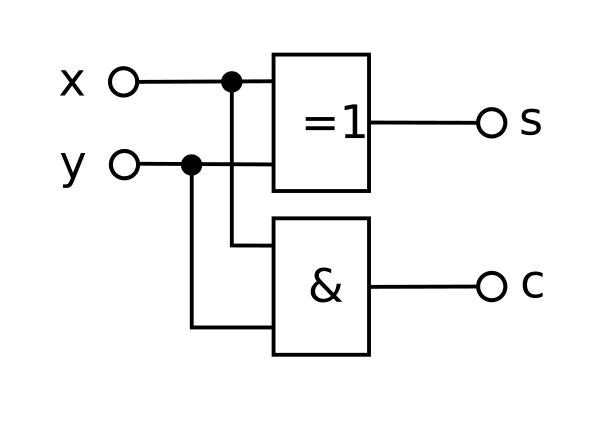
\includegraphics{images/Halbaddierer.png}
	\caption{Halbaddierer}
\end{figure}

Der \begriff{Volladdierer} besteht aus 2 Halbaddierern. Die Summe $s$ ist hier: $s=a\overline{b}\overline{c_{in}}+\overline{a}b\overline{c_{in}}+\overline{a}\overline{b}c_{in}abc_{in}+a\oplus b\oplus c_{in}$. Der Übertrag ist $c_{out}=ab+ac_{in}+bc_{in}$.

\begin{figure}[ht]
	\centering
	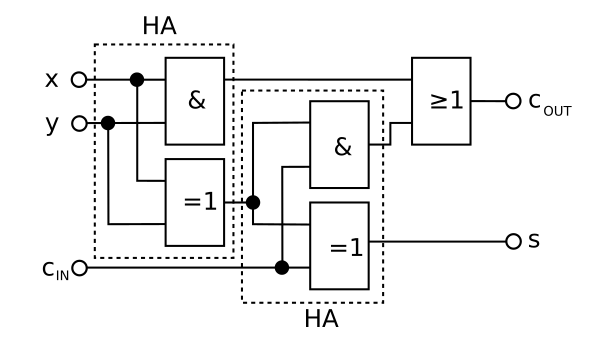
\includegraphics{images/Volladdierer.png}
	\caption{Volladdierer}
\end{figure}

Mit dem \begriff{Carry-Ripple-Adder} kann man dann endlich zwei $n$-stellige Zahlen addieren:
\begin{itemize}
	\item $a=[a_{n-1}a_{n-2}...a_1a_0]_2$
	\item $b=[b_{n-1}b_{n-2}...b_1b_0]_2$
\end{itemize}

\begin{figure}[ht]
	\centering
	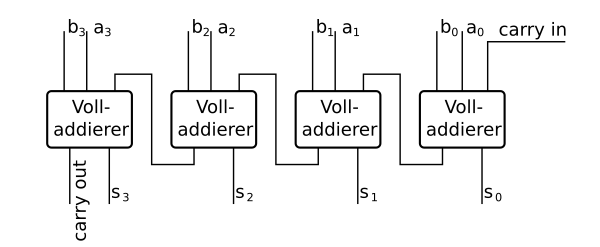
\includegraphics{images/Carry-Ripple-Adder.png}
	\caption{Carry-Ripple-Adder}
\end{figure}
$\Rightarrow T(n)=\mathcal{O}(n\cdot T_{FA})$

Machen wir zum Schluss noch eine Übertragsanalyse: Eine Bitposition $i\in\{0,1,...,n-1\}$ kann 3 verschiedene Übertragsfälle annehmen:
\begin{enumerate}
	\item kein Übertrag möglich, wenn $a_i=b_i=0$
	\item Übertrag wird weitergeleitet (\begriff{carry propergate}) $p=a_i\oplus b_i$
	\item Übertrag wird auf jeden Fall generiert (\begriff{generate bit}) $g=a_i\cdot b_i$
\end{enumerate}

Rekursionsbeziehung:
\begin{align}
	c_{i+1} &= g_i+p_i\cdot c_i=a_ib_i+(a_i\oplus b_i)c_i=a_ib_i+(a_i+b_i)c_i \notag \\
	c_{i+1} &= \underbrace{g_i+p_ig_{i-1}+p_ip_{i-1}g_{i-2}+...+p_ip_{i-1}...p_1g_0}_{G_{0,i}} + \underbrace{p_ip_{i-1}...p_1p_0}_{P_{0,i}}\cdot c_0\notag
\end{align}
\section{Subtraktion $n$-stelliger ganzer Zahlen}

Wir wollen möglichst die gleiche Hardware für die Subtraktion wie für die Addition verwenden. Dabei können wir uns zu Nutze machen, dass gilt:
\begin{align}
	a-b=a+\underbrace{(-b)}_{\text{2er Komplement}}=a+\underbrace{(\overline{b})}_{\text{1er Komplement}}+1\notag
\end{align}
Damit wird auch in der hinteren Postion ein Volladdierer benötigt und Addition und Subtraktion laufen über die gleiche Hardware.

Zugleich optimieren wir noch die Addierer. Vom Carry-Ripple-Adder zum \begriff{Carry-Lookahead-Adder} und dann zum \begriff{Carry-Skip-Adder}. Während der Carry-Ripple-Adder eine Komplexität von $T(n)=\mathcal{O}(n)$ hat, hat der Carry-Lookahead-Adder eine Komplexität von $T(n)=\mathcal{O}(\log_2 n)$

\begin{figure}[ht]
	\centering
	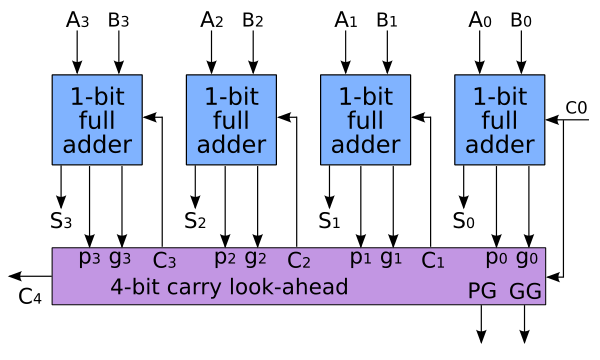
\includegraphics[width=10cm]{images/Carry-Lookahead-Adder_2.png}
	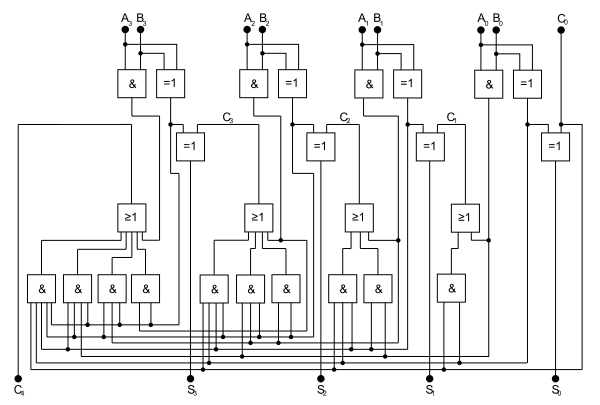
\includegraphics[width=10cm]{images/Carry-Lookahead-Adder.png}
	\caption{Carry-Lookahead-Adder}
\end{figure}

\begin{figure}[ht]
	\centering
	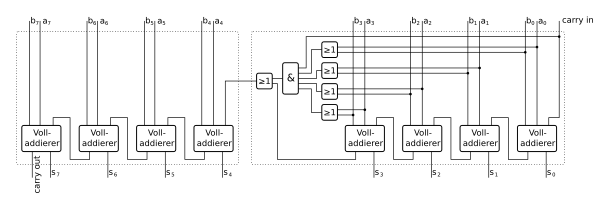
\includegraphics[width=10cm]{images/Carry-Skip-Adder.png}
	\caption{Carry-Skip-Adder}
\end{figure}
\section{Multiplikation $n$-stelliger ganzer Zahlen}

Zuerst müssen wir uns mit dem sogenannten \begriff{Shifting} beschäftigen. Shifting ist ein Vorgang, der das Bitmuster einer Zahl verschiebt. Man unterscheidet 4 Arten des Shifting:
\begin{itemize}
	\item \begriff[Shifting!]{logischer Links-Shift} $\texttt{LSHIFT}_1(a)$: verschiebt das Bitmuster von $a$ um 1 Zeichen nach links, $a_k$ fliegt raus, es werden Nullen eingefügt.
	\item \begriff[Shifting!]{logischer Rechts-Shift} $\texttt{RSHIFT}_1(a)$: verschiebt das Bitmuster von $a$ um 1 Zeichen nach rechts, $a_0$ fliegt raus, es werden Nullen eingefügt.
	\item \begriff[Shifting!]{arithmetischer Links-Shift} $\texttt{ALSHIFT}_1(a)$: verschiebt das Bitmuster von $a$ um 1 Zeichen nach links, $a_k$ fliegt raus, es wird der Wert des rechtesten Bits eingefügt.
	\item \begriff[Shifting!]{arithmetischer Rechts-Shift} $\texttt{ARSHIFT}_1(a)$: verschiebt das Bitmuster von $a$ um 1 Zeichen nach rechts, $a_0$ fliegt raus, es wird der Wert des linkesten Bits eingefügt.
\end{itemize}

Man kann die Multiplikation $a\cdot b$ auch als wiederholte Summation auffassen: $\sum\limits_{i=0}^{n-1} a_i\cdot 2^i\cdot b$. In heutigen Rechnern sind allerdings Addition und Multiplikation gleich schnell. Man kann diese wiederholte Addition aber auch deutlich verbessern:
\begin{itemize}
	\item Gruppe von $k$ Nullen in $a$: sofortiger $\texttt{ARShift}_k(a)$
	\item Gruppe von $k$ Einsen in $a$: $a=[\dots 0\underbrace{\overbrace{1}^{i}\dots\overbrace{1}^{j}}_k0\dots]$. Dann
	\begin{align}
		\sum_{i=j}^{l} 2^i = 2^{l+1}-2^j=2^{j+k}-2^j\notag
	\end{align}
\end{itemize}

Der \begriff{\person{Booth}-Algorithmus} ist eine andere Art der Optimierung. Die Idee ist, dass $a\cdot b$ mit $b=c-d$ $a\cdot b=a\cdot c-a\cdot d$ ergibt. Dazu muss der erste Faktor kodiert werden: Dazu sei $Y=[y_{n-1}\dots y_0]_2$ der zu kodierende Operand. An diesen fügt man eine weitere Stelle $y_{-1}=0$ ein. Der kodierte Operand $Y'=[y'_{n-1}\dots y'_0y_{-1}]_2$ und wir mit $y'_i=y_{i-1}-y_i$ berechnet.

Um den \person{Booth}-Algorithmus zu zeigen, wollen wir $[44]_{10}=[00101100]_2$ mit $[17]_{10}=[00010001]_2$ multiplizieren: \\
\begin{tabularx}{\textwidth}{XXXXXXXXXXXXXXXXX|p{3.2cm}}
	 &
	 &
	\cellcolor{lightgray} & \cellcolor{lightgray} & \cellcolor{lightgray} & \cellcolor{lightgray} & \cellcolor{lightgray} & \cellcolor{lightgray} & \cellcolor{lightgray} &
	\cellcolor{gray} 0 &
	\cellcolor{gray} 0 &
	\cellcolor{gray} 0 &
	\cellcolor{gray} 1 &
	\cellcolor{gray} 0 &
	\cellcolor{gray} 0 &
	\cellcolor{gray} 0 &
	\cellcolor{gray} 1 &
	\tiny 2. Faktor \\
	$\cdot$ &
	 &
	\cellcolor{lightgray} & \cellcolor{lightgray} & \cellcolor{lightgray} & \cellcolor{lightgray} & \cellcolor{lightgray} & \cellcolor{lightgray} & \cellcolor{lightgray} &
	\cellcolor{gray} 0 &
	\cellcolor{gray} 1 &
	\cellcolor{gray} -1 &
	\cellcolor{gray} 1 &
	\cellcolor{gray} 0 &
	\cellcolor{gray} -1 &
	\cellcolor{gray} 0 &
	\cellcolor{gray} 0 &
	\tiny Kodierung 1. Faktor \\
	\hline
	+ &
	&
	\cellcolor{lightgray} 0& \cellcolor{lightgray} 0& \cellcolor{lightgray} 0& \cellcolor{lightgray} 0& \cellcolor{lightgray} 0& \cellcolor{lightgray} 0& \cellcolor{lightgray} 0&
	0 &
	0 &
	0 &
	0 &
	0 &
	0 &
	0 &
	0 &
	\tiny keine Addition \\
	+ &
	&
	\cellcolor{lightgray} 0& \cellcolor{lightgray} 0& \cellcolor{lightgray} 0& \cellcolor{lightgray} 0& \cellcolor{lightgray} 0& \cellcolor{lightgray} 0& 
	0 &
	0 &
	0 &
	0 &
	0 &
	0 &
	0 &
	0 &
	\cellcolor{lightgray} &
	\tiny keine Addition \\
	+ &
	&
	\cellcolor{lightgray} 1& \cellcolor{lightgray} 1& \cellcolor{lightgray} 1& \cellcolor{lightgray} 1& \cellcolor{lightgray} 1&
	1 & 
	1 &
	1 &
	1 &
	1 &
	1 &
	1 &
	1 &
	\cellcolor{lightgray} &
	\cellcolor{lightgray} &
	\tiny 2er Komplement (2. Faktor) \\
	+ &
	&
	\cellcolor{lightgray} 0& \cellcolor{lightgray} 0& \cellcolor{lightgray} 0& \cellcolor{lightgray} 0&
	0 &
	0 & 
	0 &
	0 &
	0 &
	0 &
	0 &
	0 &
	\cellcolor{lightgray} &
	\cellcolor{lightgray} &
	\cellcolor{lightgray} &
	\tiny keine Addition \\
	+ &
	&
	\cellcolor{lightgray} 0& \cellcolor{lightgray} 0& \cellcolor{lightgray} 0&
	0 &
	0 &
	0 & 
	1 &
	0 &
	0 &
	0 &
	1 &
	\cellcolor{lightgray} &
	\cellcolor{lightgray} &
	\cellcolor{lightgray} &
	\cellcolor{lightgray} &
	\tiny 2. Faktor \\
	+ &
	&
	\cellcolor{lightgray} 1& \cellcolor{lightgray} 1&
	1 &
	1 &
	1 &
	1 & 
	1 &
	1 &
	1 &
	1 &
	\cellcolor{lightgray} &
	\cellcolor{lightgray} &
	\cellcolor{lightgray} &
	\cellcolor{lightgray} &
	\cellcolor{lightgray} &
	\tiny 2er Komplement (2. Faktor) \\
	+ &
	&
	\cellcolor{lightgray} 0&
	0 &
	0 &
	0 &
	1 &
	0 & 
	0 &
	0 &
	1 &
	\cellcolor{lightgray} &
	\cellcolor{lightgray} &
	\cellcolor{lightgray} &
	\cellcolor{lightgray} &
	\cellcolor{lightgray} &
	\cellcolor{lightgray} &
	\tiny 2. Faktor \\
	+ &
	&
	0 &
	0 &
	0 &
	0 &
	0 &
	0 & 
	0 &
	0 &
	\cellcolor{lightgray} &
	\cellcolor{lightgray} &
	\cellcolor{lightgray} &
	\cellcolor{lightgray} &
	\cellcolor{lightgray} &
	\cellcolor{lightgray} &
	\cellcolor{lightgray} &
	\tiny keine Addition \\
	\hline
	\cellcolor{lightgray} 1 &
	\cellcolor{lightgray} 0&
	\cellcolor{gray} 0 &
	\cellcolor{gray} 0 &
	\cellcolor{gray} 0 &
	\cellcolor{gray} 0 &
	\cellcolor{gray} 0 &
	\cellcolor{gray} 1 & 
	\cellcolor{gray} 0 &
	\cellcolor{gray} 1 &
	\cellcolor{gray} 1 &
	\cellcolor{gray} 1 &
	\cellcolor{gray} 0 &
	\cellcolor{gray} 1 &
	\cellcolor{gray} 1 &
	\cellcolor{gray} 0 &
	\cellcolor{gray} 0 &
	\tiny Ergebnis ohne Überlauf \\
	\hline
	= &
	 &
	\cellcolor{gray} &
	\cellcolor{gray} &
	\cellcolor{gray} &
	\cellcolor{gray} &
	\cellcolor{gray} &
	\cellcolor{gray} 1 & 
	\cellcolor{gray} 0 &
	\cellcolor{gray} 1 &
	\cellcolor{gray} 1 &
	\cellcolor{gray} 1 &
	\cellcolor{gray} 0 &
	\cellcolor{gray} 1 &
	\cellcolor{gray} 1 &
	\cellcolor{gray} 0 &
	\cellcolor{gray} 0 &
	\tiny Ergebnis mit Überlauf \\
\end{tabularx}

Dazu noch ein paar Bemerkungen:
\begin{itemize}
	\item Statt also mit $[0100000]_2$, $[0001000]_2$ und $[0000100]_2$ zu multiplizieren und die Ergebnisse zu addieren, wird nun also mit $[1000000]_2$, $[0100000]_2$, $[0010000]_2$ und $[0000100]_2$ multipliziert und die Ergebnisse addiert bzw. subtrahiert.
	\item Wie man am Beispiel sieht, kann sich die Anzahl der Additionen auch erhöhen (im Beispiel von 3 auf 4), was aber eigentlich nicht gewünscht ist. Im statistischen Durchschnitt werden im \person{Booth}-Verfahren genauso viele Additionen gebraucht wie ohne \person{Booth}-Verfahren. Der Vorteil liegt aber darin, dass in der Informatik keine Gleichverteilung von Zahlen vorliegt. Vielmehr gibt es häufig Zahlen mit vielen Nullen und durch das Zweierkomplement bei negativen Zahlen häufig viele Einsen am Anfang. Nur durch diese Tatsache hat das \person{Booth}-Verfahren Vorteile gegenüber einer normalen Multiplikation.
	\item Das Verfahren produziert das richtige Ergebnis: $44\cdot 17=[748]_{10}=[1011101100]_2$.
\end{itemize}

Die 3. Möglichkeit die Multiplikation zu verbessern, ist der \begriff{\person{Wallace}-Tree}. Die Idee dahinter ist folgende:
\begin{align}
	\underbrace{\left(\sum_{k=0}^{n} a_k2^k\right)}_{\text{Binärdarstellung }a}\cdot \underbrace{\left(\sum_{k=0}^{n} b_k2^k\right)}_{\text{Binärdarstellung }b} = \sum_{k=0}^{2n}\sum_{i+j=k} a_ib_j2^k\notag
\end{align}

Der \person{Wallace}-Tree-Multiplizierer geht in 3 Schritten vor:
\begin{enumerate}
	\item Berechne für jedes Paar $(i,j)$ mit $1\le i\le n$ und $1\le j\le k$ das Partialprodukt $a_ib_j2^{i+j}$.
	\item Addiere die Resultate dieser Berechnung innerhalb der für den \person{Wallace}-Tree-Multiplizierer spezifischen Baumstruktur stufenweise mithilfe von Voll- und Halbaddierern, bis nur noch 2 Zahlen übrig sind, die addiert werden müssen.
	\item Addiere diese beiden Zahlen mit einem normalen Addierwerk (Carry-Lookahead-Adder).
\end{enumerate}

Der \person{Wallace}-Tree benutzt den Carry-Save-Adder (CSA), der 3 Zahlen addieren kann und 2 Zahlen ausgibt: Die Sequenz der Partialsummen und die Sequenz der Übertragsbits $\to$ 2 gleich lange Zahlen

\begin{figure}[ht]
	\centering
	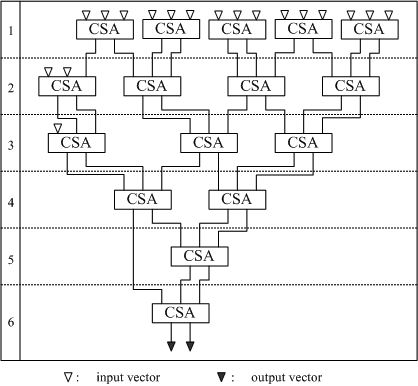
\includegraphics[width=10cm]{images/Wallace-Tree.png}
	\caption{\person{Wallace}-Tree}
\end{figure}

Die Komplexität des \person{Wallace}-Tree ist $T(n)=\mathcal{O}(\log n)$, also in etwa genau so lange wie die Addition!

\part*{Anhang}
\addcontentsline{toc}{part}{Anhang}
\appendix

%\printglossary[type=\acronymtype]

\printindex

\end{document}
